% Generated by Sphinx.
\def\sphinxdocclass{report}
\documentclass[letterpaper,10pt,oneside]{sphinxmanual}
\usepackage[utf8]{inputenc}
\DeclareUnicodeCharacter{00A0}{\nobreakspace}
\usepackage{cmap}
\usepackage{fourier}
\usepackage[T1]{fontenc}
\usepackage[spanish]{babel}
\usepackage{times}
\usepackage[Bjarne]{fncychap}
\usepackage{longtable}
\usepackage{sphinx}
\usepackage{multirow}
\usepackage{amsmath}
\usepackage{amssymb}
\usepackage{amsthm}
\usepackage{enumerate}
\usepackage{tabularx}
\usepackage{graphicx}
\usepackage{multicol}

\DeclareGraphicsExtensions{.jpg, .pdf, .png, .gif, .jpeg}

\theoremstyle{plain}%Rotulo en negrilla y texto en italicas
\newtheorem{definicion}{Definicíon}[chapter]
\newtheorem{teorema}{Teorema}[chapter]
\newtheorem{proposicion}{Proposicíon}[chapter]
\newtheorem{postulado}{Postulado}[chapter]

\theoremstyle{definition}%Rotulo en negrilla y texto normal
\newtheorem{ejemplo}{Ejemplo}[chapter]
\newtheorem{ejercicio}{Ejercicio}[chapter]

\theoremstyle{remark}%Rotulo en italicas y texto normal
\newtheorem{comentario}{Comentario}[chapter]

\newcommand{\modulo}[1]{\left | #1 \right |}
\newcommand{\modulop}[2]{\left | #1 \right |^{#2}}
\newcommand{\parcial}[2]{\fracd{\partial #1}{\partial #2}}
\newcommand{\derivada}[2]{\frac{d #1}{d#2}}
\newcommand{\derivadan}[3]{\frac{d^{#3} #1}{d#2^{#3}}}
\newcommand{\evaluar}[2]{\left. #1 \right | _{#2}}
\newcommand{\f}[3]{#1 \negthickspace : #2 \to #3}
\newcommand{\oneI}{1\hspace{-0.1cm}{\rm I}}
\newcommand{\dis}[1]{$\displaystyle{#1}$}

\DeclareMathOperator{\sen}{sen}

\def\nl{\par\noindent} %Para alineacion de parrafos
%\renewcommand{\chaptermark}[1]{\markboth{#1}{}}
%\lhead{\fancyplain{}{\bfseries\rightmark}}
%\rhead{\fancyplain{}{\bfseries\leftmark}}
\cfoot{\bfseries\thepage}

\newcommand{\Hrule}{\rule{\linewidth}{1mm}}


\title{Interactive-Numeric Documentation}
\date{March 16, 2015}
\release{1.2}
\author{Semillero de Fisica Teorica y Computacional}
\newcommand{\sphinxlogo}{}
\renewcommand{\releasename}{Release}
\makeindex

\makeatletter
\def\PYG@reset{\let\PYG@it=\relax \let\PYG@bf=\relax%
    \let\PYG@ul=\relax \let\PYG@tc=\relax%
    \let\PYG@bc=\relax \let\PYG@ff=\relax}
\def\PYG@tok#1{\csname PYG@tok@#1\endcsname}
\def\PYG@toks#1+{\ifx\relax#1\empty\else%
    \PYG@tok{#1}\expandafter\PYG@toks\fi}
\def\PYG@do#1{\PYG@bc{\PYG@tc{\PYG@ul{%
    \PYG@it{\PYG@bf{\PYG@ff{#1}}}}}}}
\def\PYG#1#2{\PYG@reset\PYG@toks#1+\relax+\PYG@do{#2}}

\expandafter\def\csname PYG@tok@nb\endcsname{\def\PYG@tc##1{\textcolor[rgb]{0.00,0.44,0.13}{##1}}}
\expandafter\def\csname PYG@tok@ow\endcsname{\let\PYG@bf=\textbf\def\PYG@tc##1{\textcolor[rgb]{0.00,0.44,0.13}{##1}}}
\expandafter\def\csname PYG@tok@sx\endcsname{\def\PYG@tc##1{\textcolor[rgb]{0.78,0.36,0.04}{##1}}}
\expandafter\def\csname PYG@tok@kd\endcsname{\let\PYG@bf=\textbf\def\PYG@tc##1{\textcolor[rgb]{0.00,0.44,0.13}{##1}}}
\expandafter\def\csname PYG@tok@nv\endcsname{\def\PYG@tc##1{\textcolor[rgb]{0.73,0.38,0.84}{##1}}}
\expandafter\def\csname PYG@tok@gt\endcsname{\def\PYG@tc##1{\textcolor[rgb]{0.00,0.27,0.87}{##1}}}
\expandafter\def\csname PYG@tok@sc\endcsname{\def\PYG@tc##1{\textcolor[rgb]{0.25,0.44,0.63}{##1}}}
\expandafter\def\csname PYG@tok@kp\endcsname{\def\PYG@tc##1{\textcolor[rgb]{0.00,0.44,0.13}{##1}}}
\expandafter\def\csname PYG@tok@ne\endcsname{\def\PYG@tc##1{\textcolor[rgb]{0.00,0.44,0.13}{##1}}}
\expandafter\def\csname PYG@tok@o\endcsname{\def\PYG@tc##1{\textcolor[rgb]{0.40,0.40,0.40}{##1}}}
\expandafter\def\csname PYG@tok@mb\endcsname{\def\PYG@tc##1{\textcolor[rgb]{0.13,0.50,0.31}{##1}}}
\expandafter\def\csname PYG@tok@ge\endcsname{\let\PYG@it=\textit}
\expandafter\def\csname PYG@tok@no\endcsname{\def\PYG@tc##1{\textcolor[rgb]{0.38,0.68,0.84}{##1}}}
\expandafter\def\csname PYG@tok@se\endcsname{\let\PYG@bf=\textbf\def\PYG@tc##1{\textcolor[rgb]{0.25,0.44,0.63}{##1}}}
\expandafter\def\csname PYG@tok@bp\endcsname{\def\PYG@tc##1{\textcolor[rgb]{0.00,0.44,0.13}{##1}}}
\expandafter\def\csname PYG@tok@nt\endcsname{\let\PYG@bf=\textbf\def\PYG@tc##1{\textcolor[rgb]{0.02,0.16,0.45}{##1}}}
\expandafter\def\csname PYG@tok@gr\endcsname{\def\PYG@tc##1{\textcolor[rgb]{1.00,0.00,0.00}{##1}}}
\expandafter\def\csname PYG@tok@go\endcsname{\def\PYG@tc##1{\textcolor[rgb]{0.20,0.20,0.20}{##1}}}
\expandafter\def\csname PYG@tok@s\endcsname{\def\PYG@tc##1{\textcolor[rgb]{0.25,0.44,0.63}{##1}}}
\expandafter\def\csname PYG@tok@nc\endcsname{\let\PYG@bf=\textbf\def\PYG@tc##1{\textcolor[rgb]{0.05,0.52,0.71}{##1}}}
\expandafter\def\csname PYG@tok@sd\endcsname{\let\PYG@it=\textit\def\PYG@tc##1{\textcolor[rgb]{0.25,0.44,0.63}{##1}}}
\expandafter\def\csname PYG@tok@il\endcsname{\def\PYG@tc##1{\textcolor[rgb]{0.13,0.50,0.31}{##1}}}
\expandafter\def\csname PYG@tok@vc\endcsname{\def\PYG@tc##1{\textcolor[rgb]{0.73,0.38,0.84}{##1}}}
\expandafter\def\csname PYG@tok@gi\endcsname{\def\PYG@tc##1{\textcolor[rgb]{0.00,0.63,0.00}{##1}}}
\expandafter\def\csname PYG@tok@sh\endcsname{\def\PYG@tc##1{\textcolor[rgb]{0.25,0.44,0.63}{##1}}}
\expandafter\def\csname PYG@tok@err\endcsname{\def\PYG@bc##1{\setlength{\fboxsep}{0pt}\fcolorbox[rgb]{1.00,0.00,0.00}{1,1,1}{\strut ##1}}}
\expandafter\def\csname PYG@tok@ni\endcsname{\let\PYG@bf=\textbf\def\PYG@tc##1{\textcolor[rgb]{0.84,0.33,0.22}{##1}}}
\expandafter\def\csname PYG@tok@gd\endcsname{\def\PYG@tc##1{\textcolor[rgb]{0.63,0.00,0.00}{##1}}}
\expandafter\def\csname PYG@tok@na\endcsname{\def\PYG@tc##1{\textcolor[rgb]{0.25,0.44,0.63}{##1}}}
\expandafter\def\csname PYG@tok@kc\endcsname{\let\PYG@bf=\textbf\def\PYG@tc##1{\textcolor[rgb]{0.00,0.44,0.13}{##1}}}
\expandafter\def\csname PYG@tok@w\endcsname{\def\PYG@tc##1{\textcolor[rgb]{0.73,0.73,0.73}{##1}}}
\expandafter\def\csname PYG@tok@gu\endcsname{\let\PYG@bf=\textbf\def\PYG@tc##1{\textcolor[rgb]{0.50,0.00,0.50}{##1}}}
\expandafter\def\csname PYG@tok@c\endcsname{\let\PYG@it=\textit\def\PYG@tc##1{\textcolor[rgb]{0.25,0.50,0.56}{##1}}}
\expandafter\def\csname PYG@tok@gs\endcsname{\let\PYG@bf=\textbf}
\expandafter\def\csname PYG@tok@nl\endcsname{\let\PYG@bf=\textbf\def\PYG@tc##1{\textcolor[rgb]{0.00,0.13,0.44}{##1}}}
\expandafter\def\csname PYG@tok@gp\endcsname{\let\PYG@bf=\textbf\def\PYG@tc##1{\textcolor[rgb]{0.78,0.36,0.04}{##1}}}
\expandafter\def\csname PYG@tok@sr\endcsname{\def\PYG@tc##1{\textcolor[rgb]{0.14,0.33,0.53}{##1}}}
\expandafter\def\csname PYG@tok@k\endcsname{\let\PYG@bf=\textbf\def\PYG@tc##1{\textcolor[rgb]{0.00,0.44,0.13}{##1}}}
\expandafter\def\csname PYG@tok@vi\endcsname{\def\PYG@tc##1{\textcolor[rgb]{0.73,0.38,0.84}{##1}}}
\expandafter\def\csname PYG@tok@kr\endcsname{\let\PYG@bf=\textbf\def\PYG@tc##1{\textcolor[rgb]{0.00,0.44,0.13}{##1}}}
\expandafter\def\csname PYG@tok@mh\endcsname{\def\PYG@tc##1{\textcolor[rgb]{0.13,0.50,0.31}{##1}}}
\expandafter\def\csname PYG@tok@sb\endcsname{\def\PYG@tc##1{\textcolor[rgb]{0.25,0.44,0.63}{##1}}}
\expandafter\def\csname PYG@tok@s2\endcsname{\def\PYG@tc##1{\textcolor[rgb]{0.25,0.44,0.63}{##1}}}
\expandafter\def\csname PYG@tok@ss\endcsname{\def\PYG@tc##1{\textcolor[rgb]{0.32,0.47,0.09}{##1}}}
\expandafter\def\csname PYG@tok@gh\endcsname{\let\PYG@bf=\textbf\def\PYG@tc##1{\textcolor[rgb]{0.00,0.00,0.50}{##1}}}
\expandafter\def\csname PYG@tok@mi\endcsname{\def\PYG@tc##1{\textcolor[rgb]{0.13,0.50,0.31}{##1}}}
\expandafter\def\csname PYG@tok@mo\endcsname{\def\PYG@tc##1{\textcolor[rgb]{0.13,0.50,0.31}{##1}}}
\expandafter\def\csname PYG@tok@vg\endcsname{\def\PYG@tc##1{\textcolor[rgb]{0.73,0.38,0.84}{##1}}}
\expandafter\def\csname PYG@tok@si\endcsname{\let\PYG@it=\textit\def\PYG@tc##1{\textcolor[rgb]{0.44,0.63,0.82}{##1}}}
\expandafter\def\csname PYG@tok@nf\endcsname{\def\PYG@tc##1{\textcolor[rgb]{0.02,0.16,0.49}{##1}}}
\expandafter\def\csname PYG@tok@m\endcsname{\def\PYG@tc##1{\textcolor[rgb]{0.13,0.50,0.31}{##1}}}
\expandafter\def\csname PYG@tok@cs\endcsname{\def\PYG@tc##1{\textcolor[rgb]{0.25,0.50,0.56}{##1}}\def\PYG@bc##1{\setlength{\fboxsep}{0pt}\colorbox[rgb]{1.00,0.94,0.94}{\strut ##1}}}
\expandafter\def\csname PYG@tok@kt\endcsname{\def\PYG@tc##1{\textcolor[rgb]{0.56,0.13,0.00}{##1}}}
\expandafter\def\csname PYG@tok@c1\endcsname{\let\PYG@it=\textit\def\PYG@tc##1{\textcolor[rgb]{0.25,0.50,0.56}{##1}}}
\expandafter\def\csname PYG@tok@nn\endcsname{\let\PYG@bf=\textbf\def\PYG@tc##1{\textcolor[rgb]{0.05,0.52,0.71}{##1}}}
\expandafter\def\csname PYG@tok@s1\endcsname{\def\PYG@tc##1{\textcolor[rgb]{0.25,0.44,0.63}{##1}}}
\expandafter\def\csname PYG@tok@mf\endcsname{\def\PYG@tc##1{\textcolor[rgb]{0.13,0.50,0.31}{##1}}}
\expandafter\def\csname PYG@tok@kn\endcsname{\let\PYG@bf=\textbf\def\PYG@tc##1{\textcolor[rgb]{0.00,0.44,0.13}{##1}}}
\expandafter\def\csname PYG@tok@nd\endcsname{\let\PYG@bf=\textbf\def\PYG@tc##1{\textcolor[rgb]{0.33,0.33,0.33}{##1}}}
\expandafter\def\csname PYG@tok@cm\endcsname{\let\PYG@it=\textit\def\PYG@tc##1{\textcolor[rgb]{0.25,0.50,0.56}{##1}}}
\expandafter\def\csname PYG@tok@cp\endcsname{\def\PYG@tc##1{\textcolor[rgb]{0.00,0.44,0.13}{##1}}}

\def\PYGZbs{\char`\\}
\def\PYGZus{\char`\_}
\def\PYGZob{\char`\{}
\def\PYGZcb{\char`\}}
\def\PYGZca{\char`\^}
\def\PYGZam{\char`\&}
\def\PYGZlt{\char`\<}
\def\PYGZgt{\char`\>}
\def\PYGZsh{\char`\#}
\def\PYGZpc{\char`\%}
\def\PYGZdl{\char`\$}
\def\PYGZhy{\char`\-}
\def\PYGZsq{\char`\'}
\def\PYGZdq{\char`\"}
\def\PYGZti{\char`\~}
% for compatibility with earlier versions
\def\PYGZat{@}
\def\PYGZlb{[}
\def\PYGZrb{]}
\makeatother

\renewcommand\PYGZsq{\textquotesingle}

\begin{document}

\maketitle
\tableofcontents
\phantomsection\label{index::doc}

\chapter{Capitulo 00: Introducción}
\label{chapter00::doc}\label{chapter00:capitulo-01-interpoladores}


\noindent Esta es la documentación oficial del proyecto cofinanciado por Colciencias desarrollado por el Semillero de Física Teórica y Computacional \href{https://sites.google.com/site/fisicatyc/home}{https://sites.google.com/site/fisicatyc/home}.

El proyecto Numéricos - Interactivos es una implementación en Python 3.4 de los métodos numéricos
elementales de Búsqueda de Raíces, Interpolación, Diferenciación e Integración.

El repositorio vigente del proyecto puede encontrarse en GitHub en el vínculo:

\href{https://github.com/fisicatyc/numericos-interactivo}{https://github.com/fisicatyc/numericos-interactivo}

Requerimientos:
\begin{quote}

El proyecto fue desarrollado utilizando las funciones Built-In de Python 3.4 por lo que no es
necesario otro tipo paquetes para su funcionamiento.
\end{quote}

El objetivo principal de este proyecto es que el usuario por medio de las herramientas facilitadas en este, encuentre un camino más interactivo para el estudio del análisis numérico. Se ***************************

\chapter[Búsqueda de Raíces]{Métodos de Búsqueda de Raíces}

\section{Métodos Cerrados}
\noindent Los métodos cerrados son métodos que requieren de dos valores iniciales para la búsqueda de
raíces, los cuales son los valores de los extremos de un intervalo que encierra una raíz. Estos
métodos siempre son convergentes pero suelen ser algo lentos.\medskip

\noindent En los métodos cerrados la metodología se puede describir como una sucesión de pasos que
cada vez acotan más el lugar de la raíz, es decir, disminuyen el tamaño del intervalo. Para
poder asegurar que una raíz se halla al interior de este intervalo debemos cumplir con que:\medskip

\begin{equation}
 f(a)f(b)\leq 0 \label{Bolz}
\end{equation}

\noindent Siendo \textit{a} y \textit{b} los extremos del intervalo actual y \textit{f} una función continua en el intervalo cerrado $\left[a,b\right]$. Si esta condición se cumple tendremos:\medskip

\[ \exists c \in \left[ a,b \right]/f(c)=0 \]
Este resultado se obtiene a partir del \textit{teorema de Bolzano}. Dado que la función es continua
recorrerá todos los valores comprendidos entre \textit{f(a)} y \textit{f(b)}, y como existe cambio de signo
entre sus extremos uno de estos valores para la función será igual a cero, por ende, entre a y b
existe una raíz.\medskip

\noindent Nótese que si la función presenta raíces de multiplicidad par (un numero par de raíces
idénticas) los métodos cerrados no convergen.\medskip

\[ \left(\lim_{a \to c^{-}}f(a)\right)\left(\lim_{b \to c^{+}}f(b)\right)> 0  \]

\noindent La diferencia entre los métodos cerrados se basa en la forma de reducir el intervalo alrededor
del cual se halla la raíz, o en otras palabras la aproximación del valor de la raíz. De ahí métodos
como búsquedas incrementales, bisección y regla falsa.\noindent

\subsection{Búsquedas Incrementales}

\noindent Los métodos de búsquedas incrementales aprovechan la característica de la ec.\ref{Bolz} para determinar el intervalo en el cuál se encuentra por lo menos una raíz, con un error igual a la mitad del tamaño de paso del avance en el intervalo. Para mejorar la precisión del método, una vez localizado el intervalo que presenta cambio de signo, este se puede subdividir en mas intervalos y nueva mente aplicar el método de búsquedas incrementales.\medskip

\noindent La formulación iterativa y el error absoluto son expresados a continuación, siendo $n$ el número de iteraciones máxima o puntos totales ($n-1$ subintervalos explorados) e $i$ el i-ésimo subintervalo (o iteración). $a$ y $b$ son los extremos del intervalo y $c$ la aproximación de la raíz.\medskip

\begin{eqnarray}
 c=a+i\frac{b-a}{n} \label{bincr}\\
 \epsilon = \frac{b-a}{2(n-1)} \nonumber
\end{eqnarray}

\subsection{Bisección}
\noindent El método de bisección es un tipo de búsqueda incremental en el que el intervalo siempre se divide en 2 subintervalos. $n$ es el número de iteraciones máxima (número de veces en que se subdividirá el intervalo).\medskip

\begin{eqnarray}
 c=\frac{a+b}{2} \label{bis}\\
 \epsilon = \frac{b-a}{2^{n+1}} \nonumber
\end{eqnarray}

\noindent Este método al igual que búsquedas incrementales, solo realizan consideraciones del intervalo mas no del comportamiento de la función en el intervalo.\medskip

\subsection{Regla Falsa}
Este método introduce a la aproximación de la raíz un conocimiento del comportamiento de la función. El hecho que un valor de la función este próximo a cero puede indicar igualmente que la posición de la variable independiente este cerca de la raíz real. Para determinar la aproximación de la raíz se unen los puntos de los extremos por una línea recta, y la intersección de esta con el eje $x$ constituye una muy buena aproximación de la raíz.\medskip

\noindent La obtención de formulación iterativa se obtiene a partir de triángulos semejantes.\medskip

\begin{equation}
\frac{f(a)}{c-a}=\frac{f(b)}{c-b} \label{regfal}
\end{equation}

\noindent Dada la consideración del comportamiento de la función tenida en regla falsa, este método en general presenta una convergencia mayor a los otros métodos cerrados. En algunos casos, el método presenta puntos de estancamiento y debe plantearse un criterio de parada adicional al error y modificar la forma iterativa del método alterando la magnitud de uno de los extremos del intervalo.\medskip

\section{Métodos Abiertos}

\noindent Los métodos abiertos son métodos cuya formulación solo requiere de un valor inicial para estimar la raíz de la función. Estos métodos no necesariamente son convergentes, pero cuando lo logran generalmente son mas rápidos que los métodos cerrados. Esta situación puede darse gracias a que los métodos abiertos toman consideraciones acerca de la geometría de la función particular que se desea.\medskip

\noindent La forma general de estos métodos es dada por la expresión ec.\ref{abierto}, donde a partir de una ecuación $f(x)=0$ se obtiene:\medskip

\begin{equation}
 x=g(x) \label{abierto} 
\end{equation}
Para que el método sea convergente se debe cumplir que en ec.\ref{abierto} 
\begin{equation}
 \modulo{g\prime(x)}<1 \label{conv}
\end{equation}
donde $g$ es una función tal que $\f{g}{\mathbb{R}}{\mathbb{R}}$

\subsection{Método de Punto Fijo}

\noindent La iteración de punto fijo exige llevar la ecuación de la forma $f(x)=0$ a la forma ec.\ref{abierto}. Una vez hecho esto, se realiza una sustitución sucesiva, teniendo la forma iterativa.\medskip

\begin{equation}
 x_{i+1}=g(x_{i}) \label{fijo}
\end{equation}

\noindent En la cual la función $g$ cumple con ec.\ref{conv}. El método de punto fijo posee convergencia lineal.\medskip

\begin{ejemplo}
\noindent Sea $f(x)=\exp^{-x}-x$, obtener la iteración de punto fijo.
\begin{eqnarray*}
 e^{-x}-x=0 \\
x_{i+1}=e^{-x_{i}}
\end{eqnarray*}
\end{ejemplo}
\begin{ejemplo}
\noindent Sea $f(x)=x^{2}-2x+3$, obtener la iteración de punto fijo.
\begin{eqnarray*}
x^{2}-2x+3=0 \\
x_{i+1}=\frac{x_{i}^{2}+3}{2}
\end{eqnarray*}
\end{ejemplo}

\subsection{Método de Newton-Raphson}

\medskip Dada una función $f(x)$ su expansión en series de Taylor alrededor de un punto $x_{0}$ puede ser expresada como:\medskip

\begin{equation}
 f(x)=f(x_{0})\evaluar{\derivada{f(x)}{x}}{x=x_{0}}(x-x_{0})+\frac{1}{2}\evaluar{\derivadan{f(x)}{x}{2}}{x=\xi}(x-x_{0})^{2} \label{taylor}
\end{equation}

\noindent Tomando el orden 1 de aproximación en ec.\ref{taylor} y despejando para $x$: \[ x=\frac{f(x)-f(x_{0})}{f\prime(x_{0})}+x_{0}\] finalmente, nos interesa la raíz de la función por lo que $f(x)=0$.\medskip

\begin{equation}
 x_{i+1}=x_{i}-\frac{f(x_{i})}{f\prime(x_{i})} \label{newton}
\end{equation}

\noindent El método de Newton, cuya iteración es descrita por la ec.\ref{newton} posee una convergencia cuadrática. El método de Newton puede tener modificaciones útiles para el caso de raíces múltiples. Así siendo $m$ la multiplicidad puede definirse la iteración como:\medskip

\begin{equation}
 x_{i+1}=x_{i}-m\frac{f(x_{i})}{f\prime(x_{i})} \label{mnewton}
\end{equation}

\noindent Otra variación del método de Newton consiste en redefinir la función a la cual se buscaran las raíces. El método tiene la forma general:\medskip

\begin{equation}
x_{i+1}=x_{i}-\frac{u(x_{i})}{u\prime(x_{i})} \label{newtonu}
\end{equation}

\noindent con $u(x)=f(x)$. Debemos proponer una función $u(x)$ tal que sus raíces sean las mismas que $f(x)$.\\
Si $f\prime(x)\neq 0$ las raíces de \[ u(x)=\frac{f(x)}{f\prime(x)}\] serán las mismas de $f(x)$. Sustituyendo esta en ec.\ref{newtonu} se obtiene la formulación de Newton modificada para raíces múltiples.\medskip

\subsection{Método de Secante}

\noindent El método de secante consiste en una alternativa al método de Newton para el calculo de la derivada de la función. Esto es ya que no siempre será posible calcular esta o dicho calculo puede constituye un costo computacional mayor, por lo que la expresión de ec.\ref{newton} se modifica incorporando una forma discreta de la derivada.\medskip

\begin{equation}
 x_{i+1}=x_{i}-\frac{f(x_{i})(x_{i-1}-x_{i})}{f(x_{i-1})-f(x_{i})} \label{secante}
\end{equation}

\noindent Es posible considerar una variante del método de secante en la cual para la aproximación de la derivada se considera un pequeño cambio en la variable independiente de la función:\medskip

\begin{equation}
x_{i+1}=x_{i}-\frac{f(x_{i})\Delta x}{f(x_{i}+\Delta x)-f(x_{i})} \label{secantem}
\end{equation}

\label{chapter01::doc}\label{chapter01:bienvenido-a-la-documentacion-de-numericos-interactivos}\label{chapter01:capitulo-01-busqueda-de-raices}

\section{Implementación del método:}

\label{chapter01:descripcion-del-metodo}

\noindent En este módulo se aplican los métodos de búsqueda de la raíces de una función, lo cual vendría a ser la búsqueda de todo elemento x que pertenezca al dominio de la función y que dicha función  cumpla f(x) = 0.\medskip

\noindent Se pretende que el usuario aplique los métodos a la solución de problemas, para lograr una mejor compresión sobre la temática y se adquieran habilidades que faciliten el progreso hacia otros métodos de mayor complejidad.\medskip

Dentro del paquete rootFinders se encuentran los siguientes métodos para la búsqueda de raíces en una función:
\begin{quote}

-Bisection Method
-FixedPoint Method
-Müller Method
-PolyRoot Method
-RegulaFalse Method
-Secant Method
\end{quote}

\section{Secuencia de llamado:}

\label{chapter01:sequencia-de-llamado}
\noindent Cada método corresponde a un archivo de extensión .py, que en el paquete se pueden encontrar como:\medskip

\begin{notice}{note}{Note:}
bisection.py, fixedpoint.py, muller.py, polyroot.py, regulafalsi.py, secant.py.
\end{notice}

Para ejecutar éstas funciones desde cualquier terminal de Python 3.4, es necesario cargar en memoria el paquete, con la línea:

\begin{notice}{note}{Note:}
from Numericos.lib.rootFinders import *
\end{notice}

Éste comando cargará simultaneamente los seis métodos del paquete. Para ejecutar un cálculo, es necesario agregar `rootFinders.(método)',
y sus respectivos argumentos. En el caso de bisección la sequencia sería:

\begin{notice}{note}{Note:}
rootFinders.bisection((`6*x-6'),-5,6,200,0.005);
\end{notice}

En el caso de cargar un único método, se utiliza el comando:

\begin{notice}{note}{Note:}
from Numericos.lib.rootFinders import muller
\end{notice}

De ésta manera solamente el método de Müller esta disponible para operar. Ésta forma simplifica la forma de llamado.


\chapter{Capitulo 02: Interpoladores}
\label{chapter02::doc}\label{chapter02:capitulo-02-interpoladores}

\noindent En general, para las aplicaciones de la ingeniería y de la investigación aplicada, sera necesario partir de información obtenida experimentalmente, lo que traduce en que la información que poseemos no es una función continua que describe el fenómeno sino de un conjunto de puntos cuya única relación inicial es que fueron obtenidos de un mismo experimento u observación de un fenómeno. El paso siguiente a partir de la obtención de estos puntos, es la obtención de una curva que describa adecuadamente los puntos (ya sea aproximándolos -curvas de regresión- o atravesándolos -curvas interpolantes-) y a partir de las cuales sea posible
construir modelos matemáticos para la descripción del fenómeno y permitan realizar predicciones acerca del mismo (al igual que estudiar el comportamiento para las condiciones no obtenidas experimentalmente). En cuanto a la interpolación, se recurre generalmente a la interpolación polinomial.\medskip

\noindent Para un conjunto de $n + 1$ puntos, existe un ubico polinomio de grado n que pasa por todos los puntos. Para construir este polinomio existen varias técnicas, como lo son Interpolación de Newton en diferencias divididas, Interpolación de Lagrange, calculo de los coeficientes directamente mediante un sistema de ecuaciones y otros. Igualmente, existen métodos de interpolación, que producen curvas suaves que pasan por todos los puntos, y que en general pueden acercarse mucho mas a la descripción del fenómeno, mas no son un polinomio, sino funciones por tramos que se constituyen de polinomios de grados bajos. Estos son los splines o trazadores.\medskip

\section{Interpolación de Newton}

Se puede formular de manera general como:

\begin{equation}
	f_n(x) = \sum\limits_{i=0}^{n}f(x_i)\prod\limits_{j=0}^{i-1}(x-x_j)
\end{equation}

Algoritmicamente es posible plantear una alternativa mediante la utilización de
diferencias divididas (lo cual no se discutirá).

\section{Interpolación de Lagrange}

El método de interpolación de Lagrange es una reformulación del método de
interpolacién de Newton (ec.3.1), que evita el cálculo de las diferencias divididas.
El polinomio resultante se puede expresar como:

\begin{equation}
	f_n(x)=\sum\limits_{i=0}^{n}L_i(x)f(x_i)
\end{equation}

donde

\begin{equation}
	L_i(x)=\prod\limits_{j=0j \neq,i}^{n}\frac{x-x_j}{x_i-x_j}
\end{equation}

La formulación de Lagrange (ec.3.2) es posible comprenderse si se observa que el
termino Li(x) a partir de ec.3.3 es 1 si x = xi y 0 para los demás puntos.

\section{Splines}

La utilización de la interpolación polinomial, al usar polinomios de grados
grandes pueden propagar errores de redondeo significativos y conducir a resultados
erróneos, además de que la existencia de puntos alejados entre si trae como
consecuencia curvas no muy bien comportadas.
En general, es de esperar que el comportamiento de un sistema no posee cambios
bruscos y se refleje por ende en curvas suaves. Para ello, se propone una alternativa
de interpolación, los splines.
Los splines o trazadores, utilizan polinomios de grados menores para interpolar
subconjuntos de puntos. Entre cada par de puntos se usa un polinomio interpolante,
y cuyas condiciones para hallar los coeficientes se establecen a partir de
condiciones de continuidad de la función y de sus primeras derivadas.
Es usual, el caso de los splines cúbicos, los cuales crean curvas suaves entre los
puntos a interpolar con oscilaciones mínimas. Los splines cúbicos, son la forma
resultante de poner una banda elástica a rodear los puntos (alfileres). Esto puede
dar idea de un principio de mínima energía, y por ende de lo apropiados que
pueden ser en la descripción de fenómenos naturales.

\section{Splines de primer grado}

Corresponde al caso mas sencillo de unión entre dos puntos, mediante el trazado de una linea recta.

\begin{equation}
	f(x)=
	\begin{cases}
	f(x_0)+m_o(x-x_0)				 & x_0\preceq,x\preceq,x_1 \\
	f(x_1)+m_1(x-x_1)				 & x_1\preceq,x\preceq,x_2 \\ 
	.&. \\
	.&. \\
	.&. \\
	f(x_{n-1})+m_{n-1}(x-x_{n-1})				 & x_{n-1}\preceq,x\preceq,x_n \\
	\end{cases}
\end{equation}

Las pendientes indicadas en ec.3.4 corresponden a 

\begin{equation}
	m_i=\frac{f(x_{i+1})-f(x_i)}{x_{i+1}-x_i}
\end{equation}

\section{Splines de segundo grado}

Los trazadores de grado superior son usuales para asegurar la continuidad de
las primeras derivadas de la función. Si se requieren m derivadas continuas, se
requiere a lo sumo de usar trazadores de grado $m + 1$.
Un trazador cuadrático asegura que la primera derivada de la función sea también
continua.
Para hallar los coeficientes se requiere de imponer condiciones que creen el conjunto
de ecuaciones iguales al número de coeficientes, de forma que el sistema sea
soluble.

\textbf{Condiciones}

La forma general del trazador para $n + 1$ datos $(i = 0..n)$ es $f_i(x) = a_ix^
2 +
b_ix+c_i$
. Estos polinomios aplican sobre los $n$ intervalos existentes entre los puntos,
y generan $3n$ coeficientes desconocidos que requieren de las siguientes condicione
para formar las $3n$ ecuaciones para solucionar el sistema de ecuaciones.

\begin{enumerate}
	\item Los valores de la función de polinomios adyacentes deben ser iguales en los
	nodos interiores. Esto es que para i = $2..n$ se da
	
	\begin{equation}
		f(x_{i-1})=a_{i-1}x^2_{i-1}+b_{i-1}x_{i-1}+c_{i-1} 
	\end{equation}
	\begin{equation}
		f(x_{i-1})=a_ix^2_{i-1}+b_ix_i+c_i
	\end{equation}
	
	Observese que por cada nodo interior se generar 2 ecuaciones, lo cual produce en total $2(n-2)$ ecuaciones.
	
	\item La primera y última función deben pasar por los puntos extremos.
	
	\begin{equation}
	f(x_0)=a_ix^2_0+b_1x_0+c_1 
	\end{equation}
	\begin{equation}
	f(x_n)=a_nx^2_n+b_nx_n+c_n
	\end{equation}
	
	Esta condición aporta 2 ecuaciones más.
	
	\item Las primeras derivadas en los nodos interiores deben ser iguales. La primera derivada en forma general se expresa como $f_i'(x)=2a_ix_{i-1}+b_i$, y por lo tanto la condición se puede expresar como
	
	\begin{equation}
		2a_{i-1}x_{i-1}+b_{i-1}=2a_ix_{i-1}+b_i
	\end{equation}
	
	Para $i=2..n, aportando n-1 ecuaciones.$
	
	\item La ecuación adicional se obtiene mediante una condición arbitrara, podemos suponer que en el primer punto la segunda derivada es cero, de donde se obtiene como ecuación, $a_1=0$. 
	
\end{enumerate}

El siguiente paso, es resolver el sistema de ecuaciones para obtener los coeficientes.

\section{Splines de tercer grado}

Para los trazadores cúbicos tenemos como expresión general $f_i(x) = a_ix^
3 +
b^
2_
i + c_ix + d_i$
. Igual que los casos anteriores, para $n + 1$ datos, existen $n$ intervalos
en los cuales se trazara un polinomio interpolante, esta vez, de grado $3$. Para los
trazadores cúbicos, se tienen $4n$ coeficientes desconocidos, y por ende se requieren
condiciones para formar el sistema de $4n$ ecuaciones necesarias para determinar
los coeficientes.

\textbf{Condiciones}

\begin{enumerate}
	\item Los valores de la función deben ser iguales en los nodos interiores. Aporta $2n-2$ ecuaciones.
	\item La primera y última función deben pasar a través de los puntos extremos. Aporta 2 ecuaciones.
	\item Las primeras derivadas en los nodos interiores deben ser iguales. Aporta $n-1$ecuaciones.
	\item Las segundas derivadas en los nodos interiores deben ser iguales. Aporta $n-1$ ecuaciones.
	\item Las segundas derivadas en los nodos extremos son cero. Aporta 2 ecuaciones.
\end{enumerate}

La condición 5 representa que la función se vuelve una linea recta en los extremos,
y esta condición particular hace que el trazador reciba la denominación de trazador
”natural”. Para los trazadores cúbicos es posible obtener una formulación que reduce el
sistema de ecuaciones de $4n$ a $n-1$, representando una considerable reducción
del costo computacional.

\section{Descripción del método:}
\label{chapter02:descripcion-del-metodo}
Este módulo se encarga de la implementación de los métodos de interpolación, que se basa en la problemática de tener n+1 puntos secuenciales,
donde x0 \textless{} x1 \textless{} x2 \textless{} x3 \textless{} ... \textless{} xn, y a partir de estos puntos diferentes se va a definir una función polinómica que pase por esos puntos.
Básicamente se está aproximando p(x)= y a una f(x)= y original, a la cual probablemente no se tiene acceso o conocimiento. Esto se hace con el fin
de modelar el comportamiento de los puntos anteriores y obtener el ``polinomio interpolante''.

Se encuentran los siguientes métodos interpoladores:
\begin{quote}

-Beziercurve Method
-Clampspline Method
-Derivpol Method
-Hermitpoly Method
-Nevilletable Method
-Newtondivdef Method
-Natspline Method
\end{quote}


\chapter{Capitulo 03: Diferenciadores}
\label{chapter03::doc}\label{chapter03:capitulo-03-diferenciadores}

\section{Diferenciación numérica}
\label{chapter03:Diferenciación numérica}

En este módulo se aplican los métodos diferenciadores o también conocidos como diferencias finitas. Se van a categorizar como diferencias centradas y no centradas, donde la primera define un conjunto de métodos numéricos en diferencias finitas con paso centrado. Y en los métodos no centrados se define un conjunto de métodos numéricos basándose en diferencias finitas SIN paso centrado.
Estas técnicas se emplean muy a menudo en análisis numérico, especialmente en ecuaciones numéricas ordinarias, ecuaciones en diferencias y ecuaciones.
En derivadas parciales. Las aplicaciones habituales suelen ser en los campos de la computación, áreas de la ingeniería térmica o en la Mecánica de fluidos.

La diferenciación numérica retoma dos elementos principales, los cambios absolutos entre dos puntos de una función real y la expansión en series de Taylor. La diferencia absoluta entre dos puntos de una función real, determina el comportamiento de la pendiente de manera local.  En el caso de una recta, la pendiente es determinada como el cociente entre las variaciones de la imagen de la función y su dominio, de la forma:

\begin{equation}
m = \frac{y_{1} - y_{0}}{x_{1} - x_{0}} = \frac{\Delta\,Y}{\Delta\,X}
\end{equation}

El comportamiento de la recta es constante respecto a los cambios en todo el dominio. En el caso de una función que posea segunda derivada, implicará la existencia de concavidades y puntos de inflexión. En éste caso el cambio a lo largo de l dominio de la función no es constante, y varía punto a punto. En ésta consideración no se considera una recta tangente a un punto, sino una recta secante entre dos puntos. Considere el caso de la figura \ref{F1}:

\begin{figure}[h]
\centering
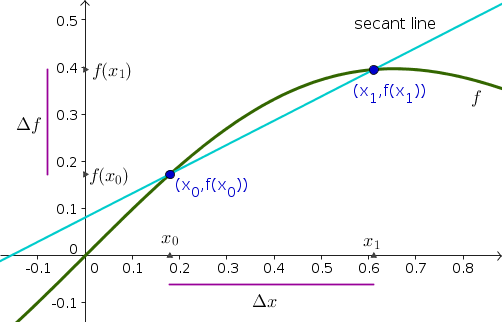
\includegraphics[scale=2]{Figures/F1.png}
\caption{Recta secante entre dos puntos de una función $f(x)$.}
\label{F1}
\end{figure}

Los puntos que forman la recta secante proveen la información de los cambio en ésta región de manera superficial, a razón que que hay muchos más cambios que no fueron mapeados. A medida que las diferencias absolutas de la imagen $\Delta\,f(x)$ y el dominio $\Delta\,X$ se reducen, los cambios mapeos se aproximan a un mapeo de un punto. De tal forma que en lugar de formar una recta secante, vuelve a parecerse como una recta tangente. Por lo que otra vez se vuelve a tener la misma forma descrita en la ecuación de la recta, obteniendo información de la pendiente en esa región. Cuando $\Delta\,f(x)\approx0$ y $\Delta\,X\approx0$, se tiene información puntual de la pendiente también conocido como el cambio instantáneo, por lo que se establece la definición de derivada:

\begin{equation}
\frac{\mathrm{d}f(x)}{\mathrm{d}x} \equiv \lim\limits_{\Delta\,X\rightarrow\,0}\frac{f(x + \Delta\,X) - f(X)}{\Delta\,X} = \lim\limits_{\Delta\,X\rightarrow\,0}\frac{\Delta\,Y}{\Delta\,X}
\end{equation}

En el mundo discreto, no existe la noción de infinitud ni continuidad. Por tanto los limites no se evalúan completamente, implicando que los puntos de nuestra función son cercanos pero siempre $\Delta\,X\approx0$ en lugar de $\Delta\,X=0$. Ésta aproximación alude a lo que se tratará en ésta sección, las diferencias finitas.\medskip

El segundo elemento que se había mencionado en el inicio, corresponde a las series de Taylor. Una de las herramientas más poderosas que se tiene en los métodos numéricos, propiamente por simplificar conceptual y matemáticamente la noción de función, entre otras ventajas. La serie de Taylor es una aproximación a una función a través de una expansión alrededor de un punto $\alpha$ utilizando las derivadas de la función, definiendo:

\begin{equation}
f(x) = \sum\limits_{n=0}^{\infty}\frac{f^{(n)}(\alpha)}{n!}(x-\alpha)^n
\end{equation}

donde $n$ corresponde a la n-ésima derivada de la función, por tanto la función a expandir ha de ser del tipo suave, diferenciable en todo el dominio. Ésta expresión tiene el significado que una función es el resultado de la suma de todos los cambios posibles de ella misma, por tanto entre más cambios se tenga de la función, es posible generar una mejor reconstrucción de la función. Al observar el comportamiento de la expansión, a medida de que se toman las derivadas de orden superior, el coeficiente que acompaña la derivada es un número que cada vez es mucho menor, por tanto los aportes a la suma son menores en magnitud para las derivadas de orden superior. Por ejemplo para la sexta derivada de la función, $6! = 720$ por tanto el aporte de ésta derivada es $720$ veces más pequeño.

Como se había mencionado anteriormente, ésta definición aplica para infinitos términos, pero en el mundo discreto ha de existir un número discreto de términos suficientes que permita aproximar la función de manera parcial. En ese caso la función se exige que sea diferenciable en el intervalo donde se realiza la expansión. A partir de ésta idea, también es posible generar aproximaciones no solamente a la función, sino también de las derivadas de la función.

Éstas aproximaciones se realizan al realizar la expansión en series de Taylor hasta un cierto término y en un punto $\alpha$ que pertenece a un intervalo $[A-B]$. Dependiendo si la serie se realiza hacia la izquierda o a la derecha de $\alpha$ se define que la expansión es hacia atrás o hacia adelante, respectivamente. Ésto define el signo en los términos de la expansión. Adicionalmente el hecho que se incluya los límites del intervalo, implica que se está tratando de con una expansión centrada. A continuación, se presenta algunas de las aproximaciones a las derivadas de una función $f(x)$.

\begin{equation}
\frac{\mathrm{d}f(x)}{\mathrm{d}x} = \frac{f(x + h) - f(x -h)}{2h} - \frac{h^2}{6}\frac{\mathrm{d}^{3}f(x)}{\mathrm{d}x^{3}}
\end{equation}

\begin{equation}
\frac{\mathrm{d}^{2}f(x)}{\mathrm{d}x^{2}} = \frac{f(x + h) - 2f(x) + f(x - h)}{h^2} + \frac{h^2}{12}\frac{\mathrm{d}^{4}f(x)}{\mathrm{d}x^{4}}
\end{equation}

\begin{equation}
\frac{\mathrm{d}^{3}f(x)}{\mathrm{d}x^{3}} \approx \frac{f(x + 2h) - 2f(x + h) + 2f(x - h) - f(x - 2h)}{2h^3} + TOS(h^2)
\end{equation}

\begin{equation}
\frac{\mathrm{d}^{4}f(x)}{\mathrm{d}x^{4}} \approx \frac{f(x + 2h) - 4f(x + h) + 6f(x) - 4f(x - h) + f(x - 2h)}{h^4} + TOS(h^2)
\end{equation}

donde $TOS(h^2)$ representa las contribuciones de los Términos de Orden Superior (TOS). Los términos con las derivas, dan indicio del orden de la expansión y del error analítico involucrado. En éste punto se puede observar lo fundamental que es el parámetro $h$ para generar las aproximaciones. Nótese que los ordenes superiores de las derivadas incluyen un factor de $h^2$, por tanto el error es menor.

Otro tipo de aproximación de las derivadas se puede realizar en el caso en que se considera un intervalo $(A-B)$, en el que no se toma los extremos del intervalo no se evalúan. Ésta aproximación se define como expansión no centrada y es de particular uso en el caso en que el intervalo a mapear es un conjunto de datos interpolados. En el caso de las dos primeras derivadas, la expansión se tiene la forma:

\begin{equation}
\frac{\mathrm{d}f(x)}{\mathrm{d}x} = \frac{f(x + h) -  f(x)}{h} + TOS(h)
\end{equation}

\begin{equation}
\frac{\mathrm{d}^{2}f(x)}{\mathrm{d}x^{2}} = \frac{f(x + 2h) -  2f(x + h) + f(x)}{h^2} + TOS(h)
\end{equation}

Nótese que éstas aproximaciones son más sencillas que la expansión centrada. Sin embargo el término de orden superior depende ahora de un $h$ con potencia de uno, implicando que hay mayor propagación de error en el truncamiento. Por tanto se sugiere que al utiliza éste tipo de expansión, utilizar valores no muy distantes para definir un adecuado valor para $h$.

La diferenciación numérica se encarga de evidenciar los cambios locales de una sección de la función definido entre dos puntos $A$ y $B$. A medida que éstos puntos se acerquen entre sí, el cambio se vuelve más local. Mientras que al alejarse éstos valores o al crecer el intervalo de diferenciación, los cambios son por secciones, pero al ser tan grandes los cambios no se mapea correctamente y por tanto la precisión de la aproximación disminuye. Ésto se puede observar en un número pequeño al elevarlo a una potencia entera, entre más grande la potencia, mucho menor se vuelve el número, pero si el número es grande, la potencia crece la magnitud. Éste número corresponde a la diferencia que hay entre éstos, definiendo $h = |A-B|$ entre más pequeño sea $h$, los errores de truncamiento y el aporte de los ordenes superiores disminuyen, en el caso contrario, el error crece exponencialmente.


\section{Descripción del método:}
\label{chapter03:descripción-del-método}

Respecto a la implementación realizada los siguientes diferenciadores, utilizan la formulación de la sección previa, para encontrar las derivadas locales de una función. La implementación también articula la expansión centrada y no centrada. En ambos casos una función analítica es ingresada como objeto lambda de python. Ésta función definida en el intervalo de derivación entre $A$ y $B$ se le asocia un valor de $h$ para generar un mapeo entre éstos puntos y calcular punto a punto las derivadas numéricas. Por tanto el resultado será una lista con éstos datos.

Adicionalmente para el caso en que se tenga los datos de una función interpolada, estos datos pueden ser utilizados para ser calcular las derivadas de éstos. Sin embargo tanto en el caso de la función como en el caso de los datos, se requiere tener en cuenta que para una mejor precisión, el intervalo de diferenciación no ha de ser muy grande y asimismo, tener presente que las derivadas de orden superior expandidas son mucho más propensas en la pérdida de precisión, que las primeras dos derivadas. Para ésto se puede utilizar valores muy cercanos o en su defecto una expansión de derivas de contengan mayores términos para ganar mayor precisión, sin embargo ésto último no es una práctica común.

A continuación los nombres de los programas:

\begin{quote}
\begin{description}
\item[{-QCDA or Fourth Centered Difference Aproximation, calculates the fourth}] \leavevmode
derivative in the interval.

\item[{-SCDA or Second Centered Difference Aproximation, calculates the second}] \leavevmode
derivative in the interval.

\item[{-TCDA or Third Centered Difference Aproximation, calculates the third}] \leavevmode
derivative in the interval.

\item[{-QCDA or Fourth Centered Difference Aproximation, calculates the fourth}] \leavevmode
derivative in the interval.

\end{description}
\end{quote}

Se encuentran los siguientes métodos diferenciadores no centrados:
\begin{quote}
\begin{description}
\item[{nfirstderv}]\leavevmode
\item[{nsecondderv}]\leavevmode
\item[{snfirstderv}]\leavevmode
\end{description}
\end{quote}


\chapter{Capitulo 04: Integradores}
\label{chapter04::doc}\label{chapter04:capitulo-04-integradores}

\section{Descripción del método:}
\label{chapter04:descripcion-del-metodo}
En este módulo se encuentran los métodos integradores que aproximan la funcion f(x) que se va a integrar por medio de polinomios interpolantes de diferentes grados, donde los métodos varían según el número de puntos o intervalo que se utilice para dicha aproximación permitiendo calcular integrales definidas.
Existen varios métodos que permiten realizar el proceso de hallar una integral defina y se dividen en este proyecto en las siguientes categorías:
\begin{quote}

\begin{optionlist}{3cm}
\item [-ClosedNewtonCotes]  
{\color{red}\bfseries{}*}Fournodescotes
{\color{red}\bfseries{}*}simprule
{\color{red}\bfseries{}*}tesimprule
{\color{red}\bfseries{}*}trapzrule
\item [-CompositeRules]  
{\color{red}\bfseries{}*}Compmidtrule
{\color{red}\bfseries{}*}compsimrule
{\color{red}\bfseries{}*}comptraprule
\item [-DoubleIntegral]  
{\color{red}\bfseries{}*}Gaussblint
{\color{red}\bfseries{}*}Simpbdlintg
\item [-OpenNewtonCotes]  
{\color{red}\bfseries{}*}Midpointrule
{\color{red}\bfseries{}*}Onenodeopn
{\color{red}\bfseries{}*}Thrnodeopn
{\color{red}\bfseries{}*}twonodeopn
\item [-Tripleintegral]  
{\color{red}\bfseries{}*}Gausstpllint
\end{optionlist}

-Adapquad
-Natspline
-Romberginted
\end{quote}


\chapter{Capitulo 05: Extrapoladores}
\label{chapter05:capitulo-05-extrapoladores}\label{chapter05::doc}

\section{Descripción del método:}
\label{chapter05:descripcion-del-metodo}
Este módulo se encarga de los métodos de extrapolación, son métodos científico lógicos, que se basan en suponer que el curso de los acontecimientos continuara, es decir, afirma que existen unos axiomas y que estos son extrapolables a una nueva situación. La base de la extrapolación son observaciones secuenciales realizados en periodos conocidos de tiempo, estas observaciones son luego registradas como variables cuantitativas, medidas con algún tipo de escala.\medskip

Se usan para buscar soluciones a problemas lógicos o enseñar la misma pedagogía, lo cual los convierte en una herramienta muy utilizada en el marco
profesional y de enseñanza, no son necesariamente exclusivos de los métodos de interpolación y tampoco se pueden considerar únicos.

En el marco de los métodos numéricos, los extrapoladores permiten recalcular, a partir de dos aproximaciones, un valor más preciso. Ésta herramienta es la piedra angular de los métodos de cuadratura. Al estar integrado en un método particular, los valores que arroja cada dos iteraciones son refinados. En la próxima iteración se obtiene una nueva aproximación que se refina con el valor extrapolado generando un valor aún más preciso.
Se cuenta con los siguientes métodos:
\begin{quote}

-Richarexpol o Extrapolación de Richardson
\end{quote}


\chapter{Documentación e Índice de los métodos - English Ver.}
\label{code::doc}\label{code:documentacion-e-indice-de-los-metodos-english-ver}

\section{adapquad.py}
\label{code:module-adapquad}\label{code:adapquad-py}\index{adapquad (module)}
Description: function adapquad is an adaptive quadrature method based on 
Simpson's rule for integration. It can also can be expanded into another 
integration technique by replacing those lines. It provides more accurate 
results by dividing the integration interval {[}a,b{]} into n subintervals, 
and again applying integration rule until achiving desired tolerance in 
each subinterval. If not met, the subinterval is divided again and the 
process is done again.
\begin{description}
\item[{Inputs: lowerlimit - float or integer - integration interval element.}] \leavevmode
upperlimit - float or integer - integration interval element.
tol\_val - float - desired error tolerance in calculated value.
n - integer - numbers of levels or subintervals to generate.
function - function type object - evaluates f(x) at x.

\end{description}

Output: app - float - defined integral aproximation.

Example line: adapquad(-2, 4, 0.005, 10, (lambda x: 4*sin(x)**2));

Dependencies: None.

Version: 1.1 for Python 3.4
\begin{description}
\item[{Definition and structure were taken from:}] \leavevmode
Richard L. Burden, J. Douglas Faires. ``Numerical Analysis'' 9th ed.
``Chapter 4 - Numerical differentiation and integration''. 
Cengage Learning. 2010. pp: 220 - 226.

\end{description}




Date: 29/12/2014.


\section{beziercurve.py}
\label{code:beziercurve-py}\label{code:module-beziercurve}\index{beziercurve (module)}
Description: function beziercurve generates an interpolation parametric
curve using a third order Hermite polynomial and a pair of nodes and
guidelines. Endpoint slope is calculated with the slope of lines
tangent to them. Therefore no second or first analytic derivative 
forms of curve is needed a priori. The fast computation of this interpolant
allows an interactive way to generate curves. Spatial coordinates are
the only requiremnt for calculation.
\begin{description}
\item[{Inputs: endpoints - list object - includes 4 float values for nodes.}] \leavevmode
leftguide - list object - includes 4 float values for left node.
rightguide - list object - includes 4 float values for right node.
n - integer - optional parameter defines number n+1 elements of list.

\end{description}

Output: beziercoeff - list object - Bezier cofficients of polynomial.
\begin{description}
\item[{Example code: endpoints = {[}{[}3.2, 2.4{]}, {[}3.6, 0.4{]}{]};}] \leavevmode
leftguide = {[}{[}2.8, 7.5{]}, {[}5.3, 6.4{]}{]};
rightguide = {[}{[}8.3, 7.5{]}, {[}1.6, 2.4{]}{]};
beziercurve (endpoints, leftguide, rightguide, n=10);

\end{description}

Dependencies: None.

Version: 1.3 for Python 3.4
\begin{description}
\item[{Definition and structure were taken from:}] \leavevmode
Richard L. Burden, J. Douglas Faires. ``Numerical Analysis'' 9th ed.
``Chapter 3 - Interpolation and Polynomial Approximation''. 
Cengage Learning. 2010. pp: 166 - 169.

\end{description}




Date: 27/12/2014.


\section{bisection.py}
\label{code:bisection-py}\label{code:module-bisection}\index{bisection (module)}
bisection.py is a function that calculates the roots of a polinomial function
using the bisection numerical method.
\begin{description}
\item[{inputs= rf ; raw function, string of the form a*x+b}] \leavevmode
a ; left range interval
b ; right range interval
n ; number of iterations
t ; tolerance of calculation

\end{description}

output= x ; the aproximated value of x such that f(x)=0

version: 1.01 for python 2.7

fast\_Code: bisection((`6*x-6'),-5,6,200,0.005);

author: JJ.Cadavid - SFTC - EAFIT University
date: 24/08/2014.


\section{clampspline.py}
\label{code:module-clampspline}\label{code:clampspline-py}\index{clampspline (module)}
Description: function clampspline generates an interpolant of third order 
polynomial. Uses knot information of first derivatives in the first and last
knot. The coefficients are solved using the tridiagonal linear system 
vectorial equation AX = B by recursion in the strictly diagonally dominant 
matrix A.
\begin{description}
\item[{Inputs: domainpnt - list object - list whose elements are x domain data.}] \leavevmode
imagepnt - list object - list whose elements are y domain data.
fstderpnt - list object - first derivative knot information, 2 elements.

\end{description}

Outputs: a, b, c, d - Automatic tuple of lists - interpolant coefficients.
\begin{description}
\item[{Example code: domainpnt = {[}0 + (x*(10-0)/5)*x**2 for x in range(6){]};}] \leavevmode
imagepnt = {[}0 + (x*(10-0)/5)*x**(2*3**0.5) for x in range(6){]};
fstderpnt = {[}{]};

\end{description}

Dependencies: None.

Version: 1.1 for Python 3.4
\begin{description}
\item[{Definition and structure were taken from:}] \leavevmode
Richard L. Burden, J. Douglas Faires. ``Numerical Analysis'' 9th ed.
``Chapter 3 - Interpolation and Polynomial Approximation''. 
Cengage Learning. 2010. pp: 153 - 156.

\end{description}




Date: 27/12/2014.


\section{compmidtrule.py}
\label{code:module-compmidtrule}\label{code:compmidtrule-py}\index{compmidtrule (module)}
Description: function compmidtrule is part of the Composite Integration
Techniques and can be thought as an upgrated version of midpoint rule
integration technique that aproximates a defined integal evaluated in {[}a,b{]}
with better presicion in larger intervals. It's truncation error is of order
h\textasciicircum{}2 and defined by a second order derivative.
\begin{description}
\item[{Inputs: lowerlimit - float - defines first limit of integration.}] \leavevmode
upperlimit - float - defines last limit of integration.
redc - integer - even integer that defines subintervals.
function - function type object - evaluates f(x) at x.

\end{description}

Outputs: integ - float - defined integral aproximation

Example line: compmidtrule(-3.15, 6.2, 500, (lambda x: 2*x**3 + 4.3));

Dependencies: None.

Version: 1.2 for Python 3.4
\begin{description}
\item[{Definitions were taken from:}] \leavevmode
Richard L. Burden, J. Douglas Faires. ``Numerical Analysis'' 9th ed.
``Chapter 4 - Numerical Differentiation and Integration''. 
Cengage Learning. 2010. pp: 203 - 209.

\end{description}




Date: 28/12/2014.


\section{compsimprule.py}
\label{code:compsimprule-py}\label{code:module-compsimprule}\index{compsimprule (module)}
Description: function compsimprule is part of the Composite Integration
Techniques and can be thought as an upgrated version of Simpson rule
integration technique that aproximates a defined integal evaluated in {[}a,b{]}
with better presicion in larger intervals. It's truncation error is of order
h\textasciicircum{}4 and defined by a fourth order derivative. Presicion is slighly better
than Composite midpoint rule and so is the best option when minimizing
number of computations. Is also known to be an all-purpose quadrature algorithm.
\begin{description}
\item[{Inputs: lowerlimit - float - defines first limit of integration.}] \leavevmode
upperlimit - float - defines last limit of integration.
redc - integer - even integer that defines subintervals
function - function type object - evaluates f(x) at x.

\end{description}

Outputs: integ - float - defined integral aproximation

Example line: integ = compsimprule(0, 2, 1000, (lambda x: 4*x**3));

Dependencies: None.

Version: 1.2 for Python 3.4
\begin{description}
\item[{Definition and structure were taken from:}] \leavevmode
Richard L. Burden, J. Douglas Faires. ``Numerical Analysis'' 9th ed.
``Chapter 4 - Numerical Differentiation and Integration''. 
Cengage Learning. 2010. pp: 203 - 209.

\end{description}


Date: 28/12/2014.


\section{comptraprule.py}
\label{code:module-comptraprule}\label{code:comptraprule-py}\index{comptraprule (module)}
Description: function comptraprule is part of the Composite Integration
Techniques and can be thought as an upgrated version of Trapezoidal rule
integration technique that aproximates a defined integal evaluated in {[}a,b{]}
with better presicion in larger intervals. It's truncation error is of order
h\textasciicircum{}2 and defined by a second order derivative. Similar to compmidtrule but
request more operations Presicion is similar to Composite midpoint rule.
Difference from the other methods is the need of only one integration interval
therefore the number of subintervals can be even or odd.
\begin{description}
\item[{Inputs: lowerlimit - float - defines first limit of integration.}] \leavevmode
upperlimit - float - defines last limit of integration.
redc - integer - integer that reduces space grid in domain.
function - function type object - evaluates f(x) at x.

\end{description}

Outputs: integ - float - defined integral aproximation

Example line: integ = comptraprule(-2, 2, 40, (lambda x: 3*x**4));

Dependencies: None.

Version: 1.2 for Python 3.4
\begin{description}
\item[{Definitions were taken from:}] \leavevmode
Richard L. Burden, J. Douglas Faires. ``Numerical Analysis'' 9th ed.
``Chapter 4 - Numerical Differentiation and Integration''. 
Cengage Learning. 2010. pp: 153 - 156.

\end{description}




Date: 28/12/2014.


\section{derivpol.py}
\label{code:module-derivpol}\label{code:derivpol-py}\index{derivpol (module)}
Description: function derivpol calculates the derivatives of interpolated
data. A good choice to create interpolant are the cubic splines they are
used in this program. Clamped and Natural Splines used information of
first and second derivatives in knots, by applying algebraic manipulation
expressions to calculate derivates are obtained.
\begin{description}
\item[{Inputs: domainlist - list object - list whose elements are x domain data.}] \leavevmode
imagelist - list object - list whose elements are y domain data.
evalpnt - list object - point to evaluate the derivatives.

\end{description}

Outputs: firstderiv, secndderiv - Automatic tuple of lists of derivatives.
\begin{description}
\item[{Example code: domainlist = {[}0 + (x*(10-0)/5)*x**2 for x in range(6){]};}] \leavevmode
imagelist = {[}0 + (x*(10-0)/5)*x**4 for x in range(6){]};
evalpnt = 5.4;
fd, sd = derivpol(domainlist, imagelist, evalpnt);

\end{description}

Dependencies: cubicSpline.py - Jaan Kiusalaasr - 2013.

Version: 1.1 for Python 3.4
\begin{description}
\item[{Definition and structure were taken from:}] \leavevmode
Jaan Kiusalaasr. ``Numerical Methods in Engineering With Python 3''.
3th ed. ``Chapter 5 - Numerical Differentiation''. 
Cambridge University Press. 2013. PP. 191 - 195.

\end{description}




Date: 28/12/2014.


\section{FCDA.py}
\label{code:module-FCDA}\label{code:fcda-py}\index{FCDA (module)}
Description: class centraldiff defines a set of numerical methods based on
finite differences of central step. Capable of aproximating derivatives at
a given point inside an interval. Central step does not evaluate derivatives
at endpoints. Precision is highly dependant on interval size, bigger intervals
lead to highter truncation errors. Minor error types are of h\textasciicircum{}2 order.
Analitical errors can be calculated using fourth derivatives. Highter
derivative orders can lead to high truncation errors, so results are likely
to differ a lot from analytical results, especially with interpolated data.

FCDA or First Centered Difference Aproximation, calculates the first
derivative in the interval. Dependencies: testlambda, getarray.
\begin{description}
\item[{Method inputs: n - integer - Defines number of n+1 elements in list.}] \leavevmode
lowerlimit - float - first term of interval.
upperlimit - float - last term of interval.
function - function type object - evaluates f(x) at x.

\end{description}

Method output: diff\_array - list - list of derivated values in (a,b).

call sequence example: centraldiff.FCDA(4, 0, 2, (lambda x: 4*sin(x)**2));

Dependencies: None.

Version: 1.2 for Python 3.4
\begin{description}
\item[{Definitions are taken from:}] \leavevmode
Jaan Kiusalaasr. ``Numerical Methods in Engineering With Python 3''.
3th ed. ``Chapter 5 - Numerical Differentiation''. 
Cambridge University Press. 2013. PP. 183 - 185.

\end{description}




Date: 28/12/2014.


\section{fixedpoint.py}
\label{code:module-fixedpoint}\label{code:fixedpoint-py}\index{fixedpoint (module)}\begin{description}
\item[{fixedpont.py finds the root of a function using the fixed point method given the}] \leavevmode
initial aproximations p0.

\item[{Inputs: g - Fixed point function with the form x=g(x) obtained from f(x)=0}] \leavevmode
p0 - Initial aproximation
tol - Tolerance
n - Maximum number of itarations

\end{description}

Outputs: Aproximate solution X or message of failure

Quick Code: fixedpoint(`(1.0/2.0)*((10.0-x**3)**(1.0/2.0))',1.5,3,10**-8)

Version: 1.0

Author: Sebastián Castaño y Felipe Lopez - SFTC - EAFIT University


\section{fournodescotes.py}
\label{code:fournodescotes-py}\label{code:module-fournodescotes}\index{fournodescotes (module)}
Description: class numecinteg is a set of numerical techniques applied to
Numerical Integration, based on the elemental Closed Newton-Cotes and
Open Newton-Cotes Formulas. This set holds the fundamental technique for
highter ones like Composite Numerical Integration and Adapatative Quadrature.
So for that extent, small integration intervals are required to achive certain
presicion. The methods described here works in a similar way by taking an
integration interval and reduced it in equally spaced elements or more 
subintervals and sum each of them. The success of this techniques is based
on parameter h, which is the space grid size. Lower spacing will grand better
presicion, also truncation and round-off error will increase by minor changes
in h, every technique differs on how it's analitical error increases.

The program set allows to input interpolated data or an analytical expression
as a lambda object. More restriction is applied to interpolated data, since
not all orders can be integrated properly with every technique. For high 
interval integration, comptechrule.py or adapquad.py set is recommended.
\begin{description}
\item[{Method Inputs: lowerlimit - float - First element in integration interval}] \leavevmode
upperlimit - float - Last element in integration interval
function - lambda object type - evaluates f(x) at x -- or
\begin{itemize}
\item {} 
list - coefficients of interpolated data

\end{itemize}

flag - integer - optional - defines 0: lambda type 1: list type

\end{description}

Method Output: integ - float - Integration aproximation

Example code: integ = newtoncotesf(0, 6, lambda x: 2*x, flag = 0);

Dependencies: None.

Version: 1.2 for Python 3.4
\begin{description}
\item[{Definitions are taken from:}] \leavevmode
Richard L. Burden, J. Douglas Faires. ``Numerical Analysis'' 9th ed.
``Chapter 4 - Numerical Differentiation and Integration''. 
Cengage Learning. 2010. pp: 193 - 201.

\end{description}




Date: 28/12/2014.


\section{gaussdblint.py}
\label{code:module-gaussdblint}\label{code:gaussdblint-py}\index{gaussdblint (module)}
Description: function gaussdblint obtains a defined double integral 
aproximation using a nested gaussian quarature. The strategy of calculation
is using the Legendre polynomials roots and coeficients. So that high grade 
polynomials can be evaluated with accuracy. Adventage of this is the no
need of equally spaced elements in domain. The function allows that the
limits of second integral can be variable as a function of the independent
variable or can be defined values. The second strategy of calculation is
the continuous calculation of the second variable space grid. Since
it can change, new grid size is created for every y value.
\begin{description}
\item[{Inputs: x\_limits - list object - list with x first integral limits}] \leavevmode
y\_limits - list object - list with y second integral limits or functions
evalpnt - list object - point to evaluate the derivatives.
m - integer - number of subintervals in y domain.
n - integer - number of subintervals in x domain.
function - function object type - a double variable lambda object.
roots - nested list - list of n, m order roots of Legendre Polynomials.
coefflist - nested list - list of n, m coefficients of L. Polynomials.
flag - integer - 0: defined y limits, 1: variable y limits. Default 0.

\end{description}

Outputs: J - float - double integration aproximation.
\begin{description}
\item[{Example code: x\_limits = {[}0, 5{]};}] \leavevmode
y\_limits = {[}0, 5{]};
m = 3;
n = 2;
function = lambda x,y: y*x*3 + y**2 - x;
roots = {[}{]};
coefflist = {[}{]};

\end{description}

Dependencies: None.

Version: 1.3 for Python 3.4
\begin{description}
\item[{Definition and structure were taken from:}] \leavevmode
Richard L. Burden, J. Douglas Faires. ``Numerical Analysis'' 9th ed.
``Chapter 4 - Numerical Differentiation and Integration''. 
Cengage Learning. 2010. pp: 240 - 244.

\end{description}




Date: 29/12/2014.


\section{gausstpllint.py}
\label{code:module-gausstpllint}\label{code:gausstpllint-py}\index{gausstpllint (module)}
Description: function gausstpllint obtains a defined triple integral 
aproximation using a nested gaussian quarature. The strategy of calculation
is using the Legendre polynomials roots and coeficients. So that high grade 
polynomials can be evaluated with accuracy. Adventage of this is the no need
of equally spaced elements in domain. The function allows that the limits of 
second or third integral can be variable as a function of the independent 
variable or can be defined values. The second strategy of calculation is 
the continuous calculation of the second variable space grid. Since it can 
change, new grid size is created for every y value and z value.
\begin{description}
\item[{Inputs: x\_limits - list object - list with x first integral limits}] \leavevmode
y\_limits - list object - list with y second integral limits or functions
z\_limits - list object - list with z second integral limits or functions
evalpnt - list object - point to evaluate the derivatives.
m - integer - number of subintervals in y domain.
n - integer - number of subintervals in x domain.
p - integer - number of subintervals in x domain.
function - function object type - a double variable lambda object.
roots - nested list - list of n, m order roots of Legendre Polynomials.
coefflist - nested list - list of n, m coefficients of L. Polynomials.
flag - integer - 0: defined y limits, 1: variable y limits. Default 0.

\end{description}

Outputs: J - float - double integration aproximation.
\begin{description}
\item[{Example code: x\_limits = {[}0, 5{]};}] \leavevmode
y\_limits = {[}0, 5{]};
m = 3;
n = 2;
function = lambda x,y: y*x*3 + y**2 - x;
roots = {[}{]};
coefflist = {[}{]};

\end{description}

Dependencies: None.

Version: 1.3 for Python 3.4
\begin{description}
\item[{Definition and structure were taken from:}] \leavevmode
Richard L. Burden, J. Douglas Faires. ``Numerical Analysis'' 9th ed.
``Chapter 4 - Numerical Differentiation and Integration''. 
Cengage Learning. 2010. pp: 245 - 246.

\end{description}




Date: 29/12/2014.


\section{hermitpoly.py}
\label{code:hermitpoly-py}\label{code:module-hermitpoly}\index{hermitpoly (module)}
Description: function hermitpoly calculates an interpolant based on Hermit
interpolation aided with devided difference. Using the first derivative 
along the domain.
\begin{description}
\item[{Inputs: domainlist - list object - list whose elements are x domain data.}] \leavevmode
imagelist - list object - list whose elements are y domain data.
derivalist - list object - list with first derivative data.

\end{description}

Outputs: hermitcoeff - list object- Hermit interpolant coefficients.
\begin{description}
\item[{Example code: domainlist = {[}0 + (x*(10-0)/5)*x**2 for x in range(6){]};}] \leavevmode
imagelist = {[}0 + (x*(10-0)/5)*x**4 for x in range(6){]};
derivalist = {[}{]};

\end{description}

Dependencies: None.

Version: 1.3 for Python 3.4
\begin{description}
\item[{Definition and structure were taken from:}] \leavevmode
Richard L. Burden, J. Douglas Faires. ``Numerical Analysis'' 9th ed.
``Chapter 3 - Interpolation and Polynomial Approximation''. 
Cengage Learning. 2010. pp: 133 - 141.

\end{description}




Date: 27/12/2014.


\section{midpointrule.py}
\label{code:module-midpointrule}\label{code:midpointrule-py}\index{midpointrule (module)}
Description: class numecinteg is a set of numerical techniques applied to
Numerical Integration, based on the elemental Closed Newton-Cotes and
Open Newton-Cotes Formulas. This set holds the fundamental technique for
highter ones like Composite Numerical Integration and Adapatative Quadrature.
So for that extent, small integration intervals are required to achive certain
presicion. The methods described here works in a similar way by taking an
integration interval and reduced it in equally spaced elements or more 
subintervals and sum each of them. The success of this techniques is based
on parameter h, which is the space grid size. Lower spacing will grand better
presicion, also truncation and round-off error will increase by minor changes
in h, every technique differs on how it's analitical error increases.

The program set allows to input interpolated data or an analytical expression
as a lambda object. More restriction is applied to interpolated data, since
not all orders can be integrated properly with every technique. For high 
interval integration, comptechrule.py or adapquad.py set is recommended.
\begin{description}
\item[{Method Inputs: lowerlimit - float - First element in integration interval}] \leavevmode
upperlimit - float - Last element in integration interval
function - lambda object type - evaluates f(x) at x -- or
\begin{itemize}
\item {} 
list - coefficients of interpolated data

\end{itemize}

flag - integer - optional - defines 0: lambda type 1: list type

\end{description}

Method Output: integ - float - Integration aproximation
\begin{description}
\item[{Example code: lowerlimit = 0;}] \leavevmode
upperlimit = 5;
function = {[}(x*(10-0)/5)*x-x for x in range(4){]};
flag = 1;
integ =                   numecinteg.midpointrule(
lowerlimit, upperlimit, function, flag = 0);

\end{description}

Dependencies: None.

Version: 1.2 for Python 3.4
\begin{description}
\item[{Definitions are taken from:}] \leavevmode
Richard L. Burden, J. Douglas Faires. ``Numerical Analysis'' 9th ed.
``Chapter 4 - Numerical Differentiation and Integration''. 
Cengage Learning. 2010. pp: 193 - 201.

\end{description}




Date: 28/12/2014.


\section{muller.py}
\label{code:module-muller}\label{code:muller-py}\index{muller (module)}
Description: function muller is a multiple polynomial root finding algorithm.
Due to method limitations functions with roots that are not simple
(Multiplicity \textgreater{} 1), Müller's technique is limitated. For that purpose use
high order quadrature or adaptative root finding algorithms. Since polynomial
roots are unique, all functions of this type, even those with complex roots,
can be easily obtained with Müller's algorithm. This program request
three seeds in which the roots are located, from there all roots there are
obatained. This program will be traslated to polyroot class to make a
selection between  Müller's and Horner's technique whether or not there are
complex roots. If tolerance is not met the program raises an exception.
\begin{description}
\item[{Inputs: polynm - lambda object type - polynomial function to be evaluated.}] \leavevmode
aprx\_list - list object - list containing three seeds.
tol - float - error tolerance in roots.
iters - integer - Positive value providing the number of loops.

\end{description}

Outputs: p - float - Polynomial root obtained from seeds.

Example code: {[}{]};

Dependencies: None.

Version: 1.2 for Python 3.4
\begin{description}
\item[{Definitions are taken from:}] \leavevmode
Richard L. Burden, J. Douglas Faires. ``Numerical Analysis'' 9th ed.
``Chapter 2 - Solutions of Equations in One Variable''. 
Cengage Learning. 2010. pp: 97 - 98.

\end{description}




Date: 24/12/2014.


\section{natspline.py}
\label{code:module-natspline}\label{code:natspline-py}\index{natspline (module)}
Description: function clampspline generates an interpolant of third order 
polynomial. Uses knot information of second derivatives in the first and last
knot. The coefficients are solved using the tridiagonal linear system 
vectorial equation AX = B by recursion in the strictly diagonally dominant 
matrix A.
\begin{description}
\item[{Inputs: domainpnt - list object - list whose elements are x domain data.}] \leavevmode
imagepnt - list object - list whose elements are y domain data.
fstderpnt - list object - second derivative knot information, 2 elements.

\end{description}

Outputs: a, b, c, d - Automatic tuple of lists - interpolant coefficients.
\begin{description}
\item[{Example code: domainpnt = {[}(x*(10-0)/5)*x**2 for x in range(6){]};}] \leavevmode
imagepnt = {[}(x*(10-0)/5)*x**(2*3**0.5) for x in range(6){]};
fstderpnt = {[}{]};

\end{description}

Dependencies: None.

Version: 1.1 for Python 3.4
\begin{description}
\item[{Definition and structure were taken from:}] \leavevmode
Richard L. Burden, J. Douglas Faires. ``Numerical Analysis'' 9th ed.
``Chapter 3 - Interpolation and Polynomial Approximation''. 
Cengage Learning. 2010. pp: 145 - 149.

\end{description}




Date: 27/12/2014.


\section{nevilletable.py}
\label{code:nevilletable-py}\label{code:module-nevilletable}\index{nevilletable (module)}
Description: function nevilletable computes a data interpolant in a recursive
way.  While Lagrange interpolation request an a priori knowledge of the n
order of interpolant, a way of reducing the computation needed to test
which polynomial order fits better is done by computing the Neville's Table.
Interpolation nodes are created in a similar way such as Newton's divided
difference. As an initial aproximation, nodes equal the f(x) data and are
slowly force to fit function behaviour by comparing the difference in first 
x data element with the following element in a forward way. Interval is set
dividing the first data with the following element, until is been completed
x data reading. When tolerance is not met, new nodes must be include or if 
so increase tolerance error.
\begin{description}
\item[{Inputs: domainpnt - list - Elements that compose data x-domain. }] \leavevmode
imagepnt - list - Elements that compose data y-domain.
tol - float - Criteria to check whether or not data fits with tolerance

\end{description}

Output: intrpnt - list - Polynomial coefficients of n-th grade
\begin{description}
\item[{Example code: domainpnt = {[}(x*(10-0)/5)+x**2 for x in range(6){]};}] \leavevmode
imagepnt = {[}(x*(10-0)/5)*x-x for x in range(6){]};
tol = 0.05;
intrpnt = nevilletable(domainpnt, imagepnt, tol);

\end{description}

Dependencies: None.

Version: 1.2 for Python 3.4
\begin{description}
\item[{Definitions are taken from:}] \leavevmode
Richard L. Burden, J. Douglas Faires. ``Numerical Analysis'' 9th ed.
``Chapter 3 - Interpolation and Polynomial Approximation''. 
Cengage Learning. 2010. pp: 117 - 123.

\end{description}




Date: 28/12/2014.


\section{newtondivdef.py}
\label{code:newtondivdef-py}\label{code:module-newtondivdef}\index{newtondivdef (module)}
Description: function newtondivdef computes a data interpolant in a recursive
way. In a similar way like Neville Table, Newton Divided difference makes
a similar approach to fit data by evaluating the function in a certain
shifted subset in domain and compare it in the non shifted place - Forward
y element respect actual position y element. In a certain way it might look
like this approach is similar to the limit definition of first derivative.
Coefficients are store in a similar 1-row way done in nevilletable. Tolerance
criteria is placed here as well, increase the number of nodes for better 
fitting or increace tolerance error.
\begin{description}
\item[{Inputs: domainpnt - list - Elements that compose data x-domain. }] \leavevmode
imagepnt - list - Elements that compose data y-domain.
tol - float - Criteria to check whether or not data fits with tolerance

\end{description}

Output: intrpnt - list - Polynomial coefficients of n-th grade
\begin{description}
\item[{Example code: domainpnt = {[}(x*(10-0)/5)+x**2 for x in range(6){]};}] \leavevmode
imagepnt = {[}(x*(10-0)/5)*x-x for x in range(6){]};
tol = 0.05;
intrpnt = nevilletable(domainpnt, imagepnt, tol);

\end{description}

Dependencies: None.

Version: 1.2 for Python 3.4
\begin{description}
\item[{Definitions are taken from:}] \leavevmode
Richard L. Burden, J. Douglas Faires. ``Numerical Analysis'' 9th ed.
``Chapter 3 - Interpolation and Polynomial Approximation''. 
Cengage Learning. 2010. pp: 124 - 126.

\end{description}




Date: 25/12/2014.


\section{nfirstderv.py}
\label{code:module-nfirstderv}\label{code:nfirstderv-py}\index{nfirstderv (module)}
Description: class ncentraldiff defines a set of numerical methods based on
finite differences with no central step - forward or backward. Capable of
aproximating derivatives at a given point inside an interval including 
endpoints. Precision is highly dependant on interval size, bigger intervals
lead to highter truncation errors. Minor error types are of h\textasciicircum{}2 order. First
non centered aproximations for derivatives are a fast way to obtain a good
aproximation, but second non centerd aproximations provides more accurate
results but increase computation demand. Other aproximations use high order
Taylor series expansion.
\begin{description}
\item[{Method inputs: n - integer - Defines number of n+1 elements in list.}] \leavevmode
lowerlimit - float - first term of interval.
upperlimit - float - last term of interval.
function - function type object - evaluates f(x) at x.

\end{description}

Method output: diff\_array - list - list of derivated values in (a,b).
\begin{description}
\item[{call sequence example: function = lambda x: 0.5*x**3+5*x*2+6*x+6.33;}] \leavevmode
nfirstderv(4, 0, 2, function);

\end{description}

Dependencies: None.

Version: 1.2 for Python 3.4
\begin{description}
\item[{Definitions are taken from:}] \leavevmode
Jaan Kiusalaasr. ``Numerical Methods in Engineering With Python 3''.
3th ed. ``Chapter 5 - Numerical Differentiation''. 
Cambridge University Press. 2013. PP. 185 - 186.

\end{description}




Date: 28/12/2014.


\section{nsecondderv.py}
\label{code:module-nsecondderv}\label{code:nsecondderv-py}\index{nsecondderv (module)}
Description: class ncentraldiff defines a set of numerical methods based on
finite differences with no central step - forward or backward. Capable of
aproximating derivatives at a given point inside an interval including 
endpoints. Precision is highly dependant on interval size, bigger intervals
lead to highter truncation errors. Minor error types are of h\textasciicircum{}2 order. First
non centered aproximations for derivatives are a fast way to obtain a good
aproximation, but second non centerd aproximations provides more accurate
results but increase computation demand. Other aproximations use high order
Taylor series expansion.
\begin{description}
\item[{Method inputs: n - integer - Defines number of n+1 elements in list.}] \leavevmode
lowerlimit - float - first term of interval.
upperlimit - float - last term of interval.
function - function type object - evaluates f(x) at x.

\end{description}

Method output: diff\_array - list - list of derivated values in (a,b).
\begin{description}
\item[{call sequence example: function = lambda x: 0.5*x**3+5*x*2+6*x+6.33;}] \leavevmode
nsecondderv(4, 0, 2, function);

\end{description}

Dependencies: None.

Version: 1.2 for Python 3.4
\begin{description}
\item[{Definitions are taken from:}] \leavevmode
Jaan Kiusalaasr. ``Numerical Methods in Engineering With Python 3''.
3th ed. ``Chapter 5 - Numerical Differentiation''. 
Cambridge University Press. 2013. PP. 185 - 186.

\end{description}




Date: 28/12/2014.


\section{onenodeopn.py}
\label{code:module-onenodeopn}\label{code:onenodeopn-py}\index{onenodeopn (module)}
Description: class numecinteg is a set of numerical techniques applied to
Numerical Integration, based on the elemental Closed Newton-Cotes and
Open Newton-Cotes Formulas. This set holds the fundamental technique for
highter ones like Composite Numerical Integration and Adapatative Quadrature.
So for that extent, small integration intervals are required to achive certain
presicion. The methods described here works in a similar way by taking an
integration interval and reduced it in equally spaced elements or more 
subintervals and sum each of them. The success of this techniques is based
on parameter h, which is the space grid size. Lower spacing will grand better
presicion, also truncation and round-off error will increase by minor changes
in h, every technique differs on how it's analitical error increases.

The program set allows to input interpolated data or an analytical expression
as a lambda object. More restriction is applied to interpolated data, since
not all orders can be integrated properly with every technique. For high 
interval integration, comptechrule.py or adapquad.py set is recommended.
\begin{description}
\item[{Method Inputs: lowerlimit - float - First element in integration interval}] \leavevmode
upperlimit - float - Last element in integration interval
function - lambda object type - evaluates f(x) at x -- or
\begin{itemize}
\item {} 
list - coefficients of interpolated data

\end{itemize}

flag - integer - optional - defines 0: lambda type 1: list type

\end{description}

Method Output: integ - float - Integration aproximation
\begin{description}
\item[{Example code: lowerlimit = 0;}] \leavevmode
upperlimit = 5;
function = {[}(x*(10-0)/5)*x-x for x in range(4){]};
flag = 1;
integ =                   numecinteg.onenodeopn(lowerlimit, upperlimit, function, flag = 0);

\end{description}

Dependencies: None.

Version: 1.2 for Python 3.4
\begin{description}
\item[{Definitions are taken from:}] \leavevmode
Richard L. Burden, J. Douglas Faires. ``Numerical Analysis'' 9th ed.
``Chapter 4 - Numerical Differentiation and Integration''. 
Cengage Learning. 2010. pp: 193 - 201.

\end{description}




Date: 28/12/2014.


\section{polyroot.py}
\label{code:polyroot-py}\label{code:module-polyroot}\index{polyroot (module)}
Description: class numecinteg is a small class type python program used as 
a prototipe algorithm. It's actual function is to represent a polynomial from
a set of coefficients. The second feature is finding it's roots by applying
Horner's algorithm.

Method Inputs: None - Input built-in function takes data from user
\begin{description}
\item[{Method Outputs: Polinomial visualization}] \leavevmode
py,pz,b0 - automatic tuple - Provides information of roots.

\end{description}

Example code: {[}{]};

Dependencies: None.

Version: 0.8 for Python 3.4
\begin{description}
\item[{Definitions are taken from:}] \leavevmode
Richard L. Burden, J. Douglas Faires. ``Numerical Analysis'' 9th ed.
``Chapter 2 - Solutions of Equations in One Variable''. 
Cengage Learning. 2010. pp: 92 - 96.

\end{description}




Date: 24/12/2014.


\section{QCDA.py}
\label{code:module-QCDA}\label{code:qcda-py}\index{QCDA (module)}
Description: class centraldiff defines a set of numerical methods based on
finite differences of central step. Capable of aproximating derivatives at
a given point inside an interval. Central step does not evaluate derivatives
at endpoints. Precision is highly dependant on interval size, bigger intervals
lead to highter truncation errors. Minor error types are of h\textasciicircum{}2 order.
Analitical errors can be calculated using fourth derivatives. Highter
derivative orders can lead to high truncation errors, so results are likely
to differ a lot from analytical results, especially with interpolated data.

QCDA or Fourth Centered Difference Aproximation, calculates the fourth
derivative in the interval. Dependencies: testlambda, getarray.
\begin{description}
\item[{Method inputs: n - integer - Defines number of n+1 elements in list.}] \leavevmode
lowerlimit - float - first term of interval.
upperlimit - float - last term of interval.
function - function type object - evaluates f(x) at x.

\end{description}

Method output: diff\_array - list - list of derivated values in (a,b).

call sequence example: centraldiff.FCDA(4, 0, 2, (lambda x: 4*sin(x)**2));

Dependencies: None.

Version: 1.2 for Python 3.4
\begin{description}
\item[{Definitions are taken from:}] \leavevmode
Jaan Kiusalaasr. ``Numerical Methods in Engineering With Python 3''.
3th ed. ``Chapter 5 - Numerical Differentiation''. 
Cambridge University Press. 2013. PP. 183 - 185.

\end{description}




Date: 28/12/2014.


\section{regulafalsi.py}
\label{code:module-regulafalsi}\label{code:regulafalsi-py}\index{regulafalsi (module)}\begin{description}
\item[{regulafalsi.py finds the root of a function continuous in an interval {[}p0,p1{]}}] \leavevmode
where f(p0) and f(p1) have opposite signs

\item[{Inputs: f- Function in terms of x}] \leavevmode
p0,p1 - Interval
tol - Tolerance
n - Maximum number of itarations

\end{description}

Outputs: Aproximate solution X or message of failure

Quick Code: fixedpoint(`(1.0/2.0)*((10.0-x**3)**(1.0/2.0))',1.5,3,10**-8)

Version: 1.0

Author: Sebastián Castaño y Felipe Lopez - SFTC - EAFIT University


\section{richarexpol.py}
\label{code:module-richarexpol}\label{code:richarexpol-py}\index{richarexpol (module)}
Description: function richarexpol is a small method that applies Richardson
Extrapolation. This technique is one of the keystones in Advance Numerical
Methods. Extrapolation allows to increase the presicion of a numerical 
result whitout increasing data nodes, whenever space grid size, h, is involve.
For this program, extrapolation receives 2 approximations of a value dependent
on h, and by setting the correct order p from analytical truncation error
high accurate results can be obtained.
\begin{description}
\item[{Inputs: P - integer - Non negative integer setting the order of correction term}] \leavevmode
firstaprx - float - first approximation of an h dependent value;
secondprx - float - second approximation of an h dependent value;

\end{description}

Method Outputs: G - float - High accurate result

Example code: {[}{]};

Dependencies: None.

Version: 1.0 for Python 3.4
\begin{description}
\item[{Definitions are taken from:}] \leavevmode
Jaan Kiusalaasr. ``Numerical Methods in Engineering With Python 3''.
3th ed. ``Chapter 5 - Numerical Differentiation''. 
Cambridge University Press. 2013. PP. 188 - 189.

\end{description}




Date: 28/12/2014.


\section{romberginteg.py}
\label{code:module-romberginteg}\label{code:romberginteg-py}\index{romberginteg (module)}
Description: function romberginteg computes an approximation of a defined
integral in {[}a,b{]}. Romberg Integration uses other minor techniques to produce
accurate results. First aproximations are obtain from one of the Newton-Cotes
Formulas and then results are improve with extrapolation techniques. Then
the process is done all over again on the subinterval section. Every loop
grid size is half for better presicion improvement.
\begin{description}
\item[{Inputs: lowerlimit - float - First element in integration interval}] \leavevmode
upperlimit - float - Last element in integration interval
subinterv - positive integer - Number of subintervals
function - lambda object type - evaluates f(x) at x

\end{description}

Outputs: R - list object - Romberg table - integration aproximation.

Example code: R = romberginteg(-3.15, 6.2, 10, (lambda x: 2*x**3 + 4.3));

Dependencies: None.

Version: 1.5 for Python 3.4
\begin{description}
\item[{Definition and structure were taken from:}] \leavevmode
Richard L. Burden, J. Douglas Faires. ``Numerical Analysis'' 9th ed.
``Chapter 4 - Numerical Differentiation and Integration''. 
Cengage Learning. 2010. pp: 213 - 218.

\end{description}




Date: 19/02/2015.


\section{SCDA.py}
\label{code:scda-py}\label{code:module-SCDA}\index{SCDA (module)}
Description: class centraldiff defines a set of numerical methods based on
finite differences of central step. Capable of aproximating derivatives at
a given point inside an interval. Central step does not evaluate derivatives
at endpoints. Precision is highly dependant on interval size, bigger intervals
lead to highter truncation errors. Minor error types are of h\textasciicircum{}2 order.
Analitical errors can be calculated using fourth derivatives. Highter
derivative orders can lead to high truncation errors, so results are likely
to differ a lot from analytical results, especially with interpolated data.

SCDA or Second Centered Difference Aproximation, calculates the second
derivative in the interval. Dependencies: testlambda, getarray.
\begin{description}
\item[{Method inputs: n - integer - Defines number of n+1 elements in list.}] \leavevmode
lowerlimit - float - first term of interval.
upperlimit - float - last term of interval.
function - function type object - evaluates f(x) at x.

\end{description}

Method output: diff\_array - list - list of derivated values in (a,b).

call sequence example: centraldiff.FCDA(4, 0, 2, (lambda x: 4*sin(x)**2));

Dependencies: None.

Version: 1.2 for Python 3.4
\begin{description}
\item[{Definitions are taken from:}] \leavevmode
Jaan Kiusalaasr. ``Numerical Methods in Engineering With Python 3''.
3th ed. ``Chapter 5 - Numerical Differentiation''. 
Cambridge University Press. 2013. PP. 183 - 185.

\end{description}




Date: 28/12/2014.


\section{secant.py}
\label{code:module-secant}\label{code:secant-py}\index{secant (module)}\begin{description}
\item[{secant.py finds the root of a function using the Secant method given the}] \leavevmode
initial aproximations p1 and p0 so that the root is a number between them

\item[{Inputs: f - Function in terms of `x'}] \leavevmode
p0,p1 - Initial aproximations
tol - Tolerance
n - maximum number of iterations

\end{description}

Outputs: Aproximate solution X or message of failure

Quick Code: secant(`math.cos(x)-x',0.5,math.pi/4,5*10**-8,20)

Version: 1.0

Author: Sebastián Castaño - SFTC - EAFIT University


\section{simpdblintg.py}
\label{code:module-simpdblintg}\label{code:simpdblintg-py}\index{simpdblintg (module)}
Description: function simpdblintg obtains a defined double integral 
aproximation using Simpson Integration Rule by reducing intervals into
subintervals. Similar to Double Legendre-Gauss Quadrature, calculations are
done from inside to outsie, using outside domain to calculate inside 
integration domain. The sum process in this method takes the results in 
three stages, the endpoints of the interval, and subinterval results, this
last one is devided on even and odd intervals. The heavy process is done
within the subintervals by continuously modifying space grid size and by
applying Simpson Rule. There is no need for use roots or coeficients from
Legendre Polynomials for approximation, making it a bit faster than the
Gauss-Legendre Quadrature, yet presicion might decrease if compare with it.
\begin{description}
\item[{Inputs: x\_limits - list object - list with x first integral limits}] \leavevmode
y\_limits - list object - list with y second integral limits or functions
evalpnt - list object - point to evaluate the derivatives.
m - integer - number of subintervals in y domain.
n - integer - number of subintervals in x domain.
function - function object type - a double variable lambda object.
flag - integer - 0: defined y limits, 1: variable y limits. Default 0.

\end{description}

Outputs: J - float - double integration aproximation.
\begin{description}
\item[{Example code: x\_limits = {[}0, 5{]};}] \leavevmode
y\_limits = {[}0, 5{]};
m = 3;
n = 2;
function = lambda x,y: y*x*3 + y**2 - x;
roots = {[}{]};
coefflist = {[}{]};

\end{description}

Dependencies: None.

Version: 1.3 for Python 3.4
\begin{description}
\item[{Definition and structure were taken from:}] \leavevmode
Richard L. Burden, J. Douglas Faires. ``Numerical Analysis'' 9th ed.
``Chapter 4 - Numerical Differentiation and Integration''. 
Cengage Learning. 2010. pp: 240 - 244.

\end{description}




Date: 29/12/2014.


\section{simprule.py}
\label{code:simprule-py}\label{code:module-simprule}\index{simprule (module)}
Description: class numecinteg is a set of numerical techniques applied to
Numerical Integration, based on the elemental Closed Newton-Cotes and
Open Newton-Cotes Formulas. This set holds the fundamental technique for
highter ones like Composite Numerical Integration and Adapatative Quadrature.
So for that extent, small integration intervals are required to achive certain
presicion. The methods described here works in a similar way by taking an
integration interval and reduced it in equally spaced elements or more 
subintervals and sum each of them. The success of this techniques is based
on parameter h, which is the space grid size. Lower spacing will grand better
presicion, also truncation and round-off error will increase by minor changes
in h, every technique differs on how it's analitical error increases.

The program set allows to input interpolated data or an analytical expression
as a lambda object. More restriction is applied to interpolated data, since
not all orders can be integrated properly with every technique. For high 
interval integration, comptechrule.py or adapquad.py set is recommended.
\begin{description}
\item[{Method Inputs: lowerlimit - float - First element in integration interval}] \leavevmode
upperlimit - float - Last element in integration interval
function - lambda object type - evaluates f(x) at x -- or
\begin{itemize}
\item {} 
list - coefficients of interpolated data

\end{itemize}

flag - integer - optional - defines 0: lambda type 1: list type

\end{description}

Method Output: integ - float - Integration aproximation
\begin{description}
\item[{Example code: lowerlimit = 0;}] \leavevmode
upperlimit = 5;
function = {[}(x*(10-0)/5)*x-x for x in range(4){]};
flag = 1;
integ =                   numecinteg.simprule(lowerlimit, upperlimit, function, flag = 0);

\end{description}

Dependencies: None.

Version: 1.2 for Python 3.4
\begin{description}
\item[{Definitions are taken from:}] \leavevmode
Richard L. Burden, J. Douglas Faires. ``Numerical Analysis'' 9th ed.
``Chapter 4 - Numerical Differentiation and Integration''. 
Cengage Learning. 2010. pp: 193 - 201.

\end{description}




Date: 28/12/2014.


\section{snfirstderv.py}
\label{code:snfirstderv-py}\label{code:module-snfirstderv}\index{snfirstderv (module)}
Description: class ncentraldiff defines a set of numerical methods based on
finite differences with no central step - forward or backward. Capable of
aproximating derivatives at a given point inside an interval including 
endpoints. Precision is highly dependant on interval size, bigger intervals
lead to highter truncation errors. Minor error types are of h\textasciicircum{}2 order. First
non centered aproximations for derivatives are a fast way to obtain a good
aproximation, but second non centerd aproximations provides more accurate
results but increase computation demand. Other aproximations use high order
Taylor series expansion.
\begin{description}
\item[{Method inputs: n - integer - Defines number of n+1 elements in list.}] \leavevmode
lowerlimit - float - first term of interval.
upperlimit - float - last term of interval.
function - function type object - evaluates f(x) at x.

\end{description}

Method output: diff\_array - list - list of derivated values in (a,b).
\begin{description}
\item[{call sequence example: function = lambda x: 0.5*x**3+5*x*2+6*x+6.33;}] \leavevmode
ncentraldiff.snfirstderv(4, 0, 2, function);

\end{description}

call sequence example: ncentraldiff.nfirstderv(4, 0, 2, (lambda x: 4*sin(x)**2));

Dependencies: None.

Version: 1.2 for Python 3.4
\begin{description}
\item[{Definitions are taken from:}] \leavevmode
Jaan Kiusalaasr. ``Numerical Methods in Engineering With Python 3''.
3th ed. ``Chapter 5 - Numerical Differentiation''. 
Cambridge University Press. 2013. PP. 185 - 186.

\end{description}




Date: 28/12/2014.


\section{TCDA.py}
\label{code:tcda-py}\label{code:module-TCDA}\index{TCDA (module)}
Description: class centraldiff defines a set of numerical methods based on
finite differences of central step. Capable of aproximating derivatives at
a given point inside an interval. Central step does not evaluate derivatives
at endpoints. Precision is highly dependant on interval size, bigger intervals
lead to highter truncation errors. Minor error types are of h\textasciicircum{}2 order.
Analitical errors can be calculated using fourth derivatives. Highter
derivative orders can lead to high truncation errors, so results are likely
to differ a lot from analytical results, especially with interpolated data.

TCDA or Third Centered Difference Aproximation, calculates the third
derivative in the interval. Dependencies: testlambda, getarray.
\begin{description}
\item[{Method inputs: n - integer - Defines number of n+1 elements in list.}] \leavevmode
lowerlimit - float - first term of interval.
upperlimit - float - last term of interval.
function - function type object - evaluates f(x) at x.

\end{description}

Method output: diff\_array - list - list of derivated values in (a,b).

call sequence example: centraldiff.FCDA(4, 0, 2, (lambda x: 4*sin(x)**2));

Dependencies: None.

Version: 1.2 for Python 3.4
\begin{description}
\item[{Definitions are taken from:}] \leavevmode
Jaan Kiusalaasr. ``Numerical Methods in Engineering With Python 3''.
3th ed. ``Chapter 5 - Numerical Differentiation''. 
Cambridge University Press. 2013. PP. 183 - 185.

\end{description}




Date: 28/12/2014.


\section{tesimprule.py}
\label{code:module-tesimprule}\label{code:tesimprule-py}\index{tesimprule (module)}
Description: class numecinteg is a set of numerical techniques applied to
Numerical Integration, based on the elemental Closed Newton-Cotes and
Open Newton-Cotes Formulas. This set holds the fundamental technique for
highter ones like Composite Numerical Integration and Adapatative Quadrature.
So for that extent, small integration intervals are required to achive certain
presicion. The methods described here works in a similar way by taking an
integration interval and reduced it in equally spaced elements or more 
subintervals and sum each of them. The success of this techniques is based
on parameter h, which is the space grid size. Lower spacing will grand better
presicion, also truncation and round-off error will increase by minor changes
in h, every technique differs on how it's analitical error increases.

The program set allows to input interpolated data or an analytical expression
as a lambda object. More restriction is applied to interpolated data, since
not all orders can be integrated properly with every technique. For high 
interval integration, comptechrule.py or adapquad.py set is recommended.
\begin{description}
\item[{Method Inputs: lowerlimit - float - First element in integration interval}] \leavevmode
upperlimit - float - Last element in integration interval
function - lambda object type - evaluates f(x) at x -- or
\begin{itemize}
\item {} 
list - coefficients of interpolated data

\end{itemize}

flag - integer - optional - defines 0: lambda type 1: list type

\end{description}

Method Output: integ - float - Integration aproximation

Example code: integ = tesimprule(0, 2, lambda x: x, 3, flag = 0);

Dependencies: None.

Version: 1.2 for Python 3.4
\begin{description}
\item[{Definitions are taken from:}] \leavevmode
Richard L. Burden, J. Douglas Faires. ``Numerical Analysis'' 9th ed.
``Chapter 4 - Numerical Differentiation and Integration''. 
Cengage Learning. 2010. pp: 193 - 201.

\end{description}




Date: 28/12/2014.


\section{thrnodeopn.py}
\label{code:module-thrnodeopn}\label{code:thrnodeopn-py}\index{thrnodeopn (module)}
Description: class numecinteg is a set of numerical techniques applied to
Numerical Integration, based on the elemental Closed Newton-Cotes and
Open Newton-Cotes Formulas. This set holds the fundamental technique for
highter ones like Composite Numerical Integration and Adapatative Quadrature.
So for that extent, small integration intervals are required to achive certain
presicion. The methods described here works in a similar way by taking an
integration interval and reduced it in equally spaced elements or more 
subintervals and sum each of them. The success of this techniques is based
on parameter h, which is the space grid size. Lower spacing will grand better
presicion, also truncation and round-off error will increase by minor changes
in h, every technique differs on how it's analitical error increases.

The program set allows to input interpolated data or an analytical expression
as a lambda object. More restriction is applied to interpolated data, since
not all orders can be integrated properly with every technique. For high 
interval integration, comptechrule.py or adapquad.py set is recommended.
\begin{description}
\item[{Method Inputs: lowerlimit - float - First element in integration interval}] \leavevmode
upperlimit - float - Last element in integration interval
function - lambda object type - evaluates f(x) at x -- or
\begin{itemize}
\item {} 
list - coefficients of interpolated data

\end{itemize}

flag - integer - optional - defines 0: lambda type 1: list type

\end{description}

Method Output: integ - float - Integration aproximation
\begin{description}
\item[{Example code: lowerlimit = 0;}] \leavevmode
upperlimit = 5;
function = {[}(x*(10-0)/5)*x-x for x in range(4){]};
flag = 1;
integ =                   numecinteg.onenodeopn(lowerlimit, upperlimit, function, flag = 0);

\end{description}

Dependencies: None.

Version: 1.2 for Python 3.4
\begin{description}
\item[{Definitions are taken from:}] \leavevmode
Richard L. Burden, J. Douglas Faires. ``Numerical Analysis'' 9th ed.
``Chapter 4 - Numerical Differentiation and Integration''. 
Cengage Learning. 2010. pp: 193 - 201.

\end{description}




Date: 28/12/2014.


\section{trapzrule.py}
\label{code:trapzrule-py}\label{code:module-trapzrule}\index{trapzrule (module)}
Description: class numecinteg is a set of numerical techniques applied to
Numerical Integration, based on the elemental Closed Newton-Cotes and
Open Newton-Cotes Formulas. This set holds the fundamental technique for
highter ones like Composite Numerical Integration and Adapatative Quadrature.
So for that extent, small integration intervals are required to achive certain
presicion. The methods described here works in a similar way by taking an
integration interval and reduced it in equally spaced elements or more 
subintervals and sum each of them. The success of this techniques is based
on parameter h, which is the space grid size. Lower spacing will grand better
presicion, also truncation and round-off error will increase by minor changes
in h, every technique differs on how it's analitical error increases.

The program set allows to input interpolated data or an analytical expression
as a lambda object. More restriction is applied to interpolated data, since
not all orders can be integrated properly with every technique. For high 
interval integration, comptechrule.py or adapquad.py set is recommended.
\begin{description}
\item[{Method Inputs: lowerlimit - float - First element in integration interval}] \leavevmode
upperlimit - float - Last element in integration interval
function - lambda object type - evaluates f(x) at x -- or
\begin{itemize}
\item {} 
list - coefficients of interpolated data

\end{itemize}

flag - integer - optional - defines 0: lambda type 1: list type

\end{description}

Method Output: integ - float - Integration aproximation

Example code: integ = trapzrule(0, 2, lambda x: 1.5*x, flag = 0);

Dependencies: None.

Version: 1.2 for Python 3.4
\begin{description}
\item[{Definitions are taken from:}] \leavevmode
Richard L. Burden, J. Douglas Faires. ``Numerical Analysis'' 9th ed.
``Chapter 4 - Numerical Differentiation and Integration''. 
Cengage Learning. 2010. pp: 193 - 201.

\end{description}




Date: 28/12/2014.


\section{twonodeopn.py}
\label{code:module-twonodeopn}\label{code:twonodeopn-py}\index{twonodeopn (module)}
Description: class numecinteg is a set of numerical techniques applied to
Numerical Integration, based on the elemental Closed Newton-Cotes and
Open Newton-Cotes Formulas. This set holds the fundamental technique for
highter ones like Composite Numerical Integration and Adapatative Quadrature.
So for that extent, small integration intervals are required to achive certain
presicion. The methods described here works in a similar way by taking an
integration interval and reduced it in equally spaced elements or more 
subintervals and sum each of them. The success of this techniques is based
on parameter h, which is the space grid size. Lower spacing will grand better
presicion, also truncation and round-off error will increase by minor changes
in h, every technique differs on how it's analitical error increases.

The program set allows to input interpolated data or an analytical expression
as a lambda object. More restriction is applied to interpolated data, since
not all orders can be integrated properly with every technique. For high 
interval integration, comptechrule.py or adapquad.py set is recommended.
\begin{description}
\item[{Method Inputs: lowerlimit - float - First element in integration interval}] \leavevmode
upperlimit - float - Last element in integration interval
function - lambda object type - evaluates f(x) at x -- or
\begin{itemize}
\item {} 
list - coefficients of interpolated data

\end{itemize}

flag - integer - optional - defines 0: lambda type 1: list type

\end{description}

Method Output: integ - float - Integration aproximation
\begin{description}
\item[{Example code: lowerlimit = 0;}] \leavevmode
upperlimit = 5;
function = {[}(x*(10-0)/5)*x-x for x in range(4){]};
flag = 1;
integ = numecinteg.onenodeopn(lowerlimit, upperlimit, function, flag = 0);

\end{description}

Dependencies: None.

Version: 1.2 for Python 3.4
\begin{description}
\item[{Definitions are taken from:}] \leavevmode
Richard L. Burden, J. Douglas Faires. ``Numerical Analysis'' 9th ed.
``Chapter 4 - Numerical Differentiation and Integration''. 
Cengage Learning. 2010. pp: 193 - 201.

\end{description}

Date: 28/12/2014.



\renewcommand{\indexname}{Python Module Index}
\begin{theindex}
\def\bigletter#1{{\Large\sffamily#1}\nopagebreak\vspace{1mm}}
\bigletter{a}
\item {\texttt{adapquad}}, \pageref{code:module-adapquad}
\indexspace
\bigletter{b}
\item {\texttt{beziercurve}}, \pageref{code:module-beziercurve}
\item {\texttt{bisection}}, \pageref{code:module-bisection}
\indexspace
\bigletter{c}
\item {\texttt{clampspline}}, \pageref{code:module-clampspline}
\item {\texttt{compmidtrule}}, \pageref{code:module-compmidtrule}
\item {\texttt{compsimprule}}, \pageref{code:module-compsimprule}
\item {\texttt{comptraprule}}, \pageref{code:module-comptraprule}
\indexspace
\bigletter{d}
\item {\texttt{derivpol}}, \pageref{code:module-derivpol}
\indexspace
\bigletter{f}
\item {\texttt{FCDA}}, \pageref{code:module-FCDA}
\item {\texttt{fixedpoint}}, \pageref{code:module-fixedpoint}
\item {\texttt{fournodescotes}}, \pageref{code:module-fournodescotes}
\indexspace
\bigletter{g}
\item {\texttt{gaussdblint}}, \pageref{code:module-gaussdblint}
\item {\texttt{gausstpllint}}, \pageref{code:module-gausstpllint}
\indexspace
\bigletter{h}
\item {\texttt{hermitpoly}}, \pageref{code:module-hermitpoly}
\indexspace
\bigletter{m}
\item {\texttt{midpointrule}}, \pageref{code:module-midpointrule}
\item {\texttt{muller}}, \pageref{code:module-muller}
\indexspace
\bigletter{n}
\item {\texttt{natspline}}, \pageref{code:module-natspline}
\item {\texttt{nevilletable}}, \pageref{code:module-nevilletable}
\item {\texttt{newtondivdef}}, \pageref{code:module-newtondivdef}
\item {\texttt{nfirstderv}}, \pageref{code:module-nfirstderv}
\item {\texttt{nsecondderv}}, \pageref{code:module-nsecondderv}
\indexspace
\bigletter{o}
\item {\texttt{onenodeopn}}, \pageref{code:module-onenodeopn}
\indexspace
\bigletter{p}
\item {\texttt{polyroot}}, \pageref{code:module-polyroot}
\indexspace
\bigletter{q}
\item {\texttt{QCDA}}, \pageref{code:module-QCDA}
\indexspace
\bigletter{r}
\item {\texttt{regulafalsi}}, \pageref{code:module-regulafalsi}
\item {\texttt{richarexpol}}, \pageref{code:module-richarexpol}
\item {\texttt{romberginteg}}, \pageref{code:module-romberginteg}
\indexspace
\bigletter{s}
\item {\texttt{SCDA}}, \pageref{code:module-SCDA}
\item {\texttt{secant}}, \pageref{code:module-secant}
\item {\texttt{simpdblintg}}, \pageref{code:module-simpdblintg}
\item {\texttt{simprule}}, \pageref{code:module-simprule}
\item {\texttt{snfirstderv}}, \pageref{code:module-snfirstderv}
\indexspace
\bigletter{t}
\item {\texttt{TCDA}}, \pageref{code:module-TCDA}
\item {\texttt{tesimprule}}, \pageref{code:module-tesimprule}
\item {\texttt{thrnodeopn}}, \pageref{code:module-thrnodeopn}
\item {\texttt{trapzrule}}, \pageref{code:module-trapzrule}
\item {\texttt{twonodeopn}}, \pageref{code:module-twonodeopn}
\end{theindex}

\renewcommand{\indexname}{Index}
\printindex
\end{document}
